\section{Experiments}
\label{sec:experiments}
The two different backbone architecture for the generation of the latent space representation of the objects and the performance of the different clustering algorithms are evaluated by hyperparameter optimization of the different parameters along the entire pipeline of the procedure is evaluated in this section.

\subsection{Baseline Algorithm}
The already existing PointNet autoencoder currently used at \ac{IPA} is used as a baseline for evaluating the performance of the proposed algorithms in this thesis. The dimension of the output of the latent space representation of the baseline algorithm is 64. As mentioned in the restrictions in Section. \ref{sec:restrictions}, usually a two-step dimensionality reduction is performed before the datasets are grouped into clusters for the two networks evaluated in this thesis because the dimension of the output of the latent space representations is too high. This is done to suppress some noise and also to escalate the procedure by faster calculation of the pairwise distance between the datapoints. But since an output dimension of 64 is not very high, two-step dimensionality reduction is not necessary. However, to make the baseline algorithm comparable with the proposed networks, one-step dimensionality reduction is performed in some cases. 

\subsubsection{Basic Study without Dimensionality Reduction}
\label{sec:pointnet_dim}
Tab. \ref{tab:basic_without_tsne} shows the results of the baseline algorithm when no dimensionality reduction technique is used. It shows the results of the basic algorithm for the clustering of 1000 datapoints. The unit of time across all the tables in this section is in seconds unless otherwise mentioned. The four clustering algorithms \ac{HDBSCAN}, k-means clustering, spectral clustering and agglomerative clustering are evaluated. The number of clusters generated by the \ac{HDBSCAN} algorithm cannot be fixed by the user and hence it is determined by the algorithm automatically. Thus, the number of clusters after the first level of the multi-level \ac{HDBSCAN} algorithm as proposed in Section. \ref{sec:clustering_algo} is 232 in this case. As mentioned in Ch. \ref{sec:restrictions} the number of clusters for the rest of the clustering algorithms is set to 175 throughout all the experiments in this section. The \ac{DBCV} score caries in the range [-1,1] with more positive results denoting better clustering of the datapoints. The reason why \ac{HDBSCAN} algorithm shoes better results as compared to other clustering algorithms is \ac{HDBSCAN} algorithm is a density based clustering algorithm. \ac{DBCV} being a density based clustering validation index is likely to give better results for density based clustering algorithms which is proven to be true in this experiment. Furthermore, theoretically \ac{HDBSCAN} is better capable of handling noises and outliers in the dataset which can also contribute to the better results as exhibited in this experiment. 
\begin{table}[H]
    \setlength\extrarowheight{10pt}
    \caption{Results of the baseline algorithm on 1000 datapoints and without any dimensionality reduction technique. }
    \centering
    \begin{tabular}{|p{50pt}|p{60pt}|p{50pt}|p{40pt}|p{50pt}|p{40pt}|}
      \toprule
      No. of datapoints & Clustering Algorithm & No. of Clusters & Clustering Time (seconds) & \ac{DBCV} score & \ac{DBCV} Time (seconds)\\
      \midrule
      \multirow{4}{1.0in}{1000} & \ac{HDBSCAN} & 232 & 0.182 & -0.189 & 297.031 \\ \cline{2-6} 
                                & k-medoids & 175	& 3.960 & -0.332 & 237.640 \\ \cline{2-6} 
                                & Spectral & 175 & 2.396 & -0.339	& 161.604 \\ \cline{2-6}
                                & Agglomerative	& 175 & 0.115 & -0.327 & 157.584  \\ 
      \bottomrule
    \end{tabular}
    \label{tab:basic_without_tsne}
\end{table}

\subsubsection{Basic Study with T-distributed Stochastic Neighbor Embedding}
Tab. \ref{tab:basic_with_tsne} shows the results of the baseline algorithm when the \ac{t-SNE} dimensionality reduction is applied. The number of components for \ac{t-SNE} could be 1, 2 or 3 as per the available scikit-learn implementation \cite{scikit-learn}. It is set to be 2 in these set of experimentations for better and easier visualization. The \ac{DBCV} score caries in the range [-1,1] with more positive results denoting better clustering of the datapoints. The results are seen to be significantly better as compared to Tab. \ref{tab:basic_without_tsne} when dimensionality reduction technique is not applied. This is because the \ac{t-SNE} algorithm tends to keep datapoints that are distant from one another in the higher dimensional space also distant datapoints even in the lower-dimensional space. This gives rise to more dense and distinct clusters thus, improving the \ac{DBCV} score. As opposed to the result in Tab.\ref{tab:basic_without_tsne}, where the \ac{DBCV} score is negative, meaning the datapoints are mostly wrongly classification, in this table it can be seen that the datapoints are mostly correctly classified. It is also to be note that the number of clusters generated by the \ac{HDBSCAN} algorithm is 286 which is a bit more as compared to the previous case. This further hints to the direction that as a result of using \ac{t-SNE}, more dense and non-overlapping clusters are formed in the dataset. 
\begin{table}[H]
    \setlength\extrarowheight{10pt}
    \caption{Results of the baseline algorithm on 1000 datapoints after applying \ac{t-SNE} dimensionality reduction. }
    \centering
    \begin{tabular}{|p{30pt}|p{30pt}|p{40pt}|p{60pt}|p{50pt}|p{40pt}|p{30pt}|p{40pt}|}
      \toprule
      No. of datapoints & \ac{t-SNE} dim	& \ac{t-SNE} time (seconds) & Clustering Algorithm & No. of Clusters & Clustering Time (seconds) & \ac{DBCV} score & \ac{DBCV} Time (seconds)\\
      \midrule
      \multirow{4}{30pt}{1000} & 2	& 3.030 & \ac{HDBSCAN}	& 286	& 0.110 & 0.0975	& 275.039 \\ \cline{2-8} 
                                & 2	& 2.777 &	k-means	& 175	& 0.191 & -0.052  	& 94.004 \\ \cline{2-8} 
                                & 2	& 3.318 & Spectral	& 175	& 3.604 & -0.064 	& 126.854 \\ \cline{2-8}
                                & 2	& 3.190 & Agglomerative	& 175	& 0.087 & -0.076	& 113.937 \\ 
      \bottomrule
    \end{tabular}
    \label{tab:basic_with_tsne}
\end{table}
\subsubsection{Basic Study with Increasing Datapoints}
\begin{table}[H]
  \setlength\extrarowheight{10pt}
  \caption{Results of the baseline algorithm on 2000 datapoints and without any dimensionality reduction technique. }
  \centering
  \begin{tabular}{|p{50pt}|p{60pt}|p{50pt}|p{40pt}|p{50pt}|p{40pt}|}
    \toprule
    No. of datapoints & Clustering Algorithm & No. of Clusters & Clustering Time (seconds) & \ac{DBCV} score & \ac{DBCV} Time (seconds)\\
    \midrule
    \multirow{4}{1.0in}{2000} & \ac{HDBSCAN}	& 436	& 0.444 & -0.234	& 2115.777 \\ \cline{2-6} 
                              & k-medoids	& 175	& 0.793 & -0.462	& 764.222 \\ \cline{2-6} 
                              & Spectral	& 175	& 20.607 & -0.617	& 749.487 \\ \cline{2-6}
                              & Agglomerative	& 175	& 0.205 & -0.502	& 756.480 \\ 
    \bottomrule
  \end{tabular}
  \label{tab:basic_2000_without_tsne}
\end{table}
As mentioned in Ch. \ref{sec:restrictions}, it is extremely inefficient to compute the \ac{DBCV} for all the datapoints in the ABC datasets \cite{Koch_2019_CVPR} as once. It is necessary to verify that the results obtained for a smaller subset of the dataset can be interpolated for the entire dataset. In other words, the results obtained for a smaller subset of the dataset generalizes the behavior of the entire dataset well. Tab. \ref{tab:basic_2000_without_tsne} shows the results of the baseline algorithm on 2000 datapoints without applying dimensionality reduction and Tab. \ref{tab:basic_2000_with_tsne} shows the results of the baseline algorithm on 2000 datapoints when \ac{t-SNE} dimensionality reduction is applied. It is observed that roughly $10\%$ of the datapoints are classified as outliers by the \ac{HDBSCAN} algorithm for all the experiments on 1000 and 2000 datapoints. 

\begin{table}[H]
    \setlength\extrarowheight{10pt}
    \caption{Results of the baseline algorithm on 2000 datapoints after applying \ac{t-SNE} dimensionality reduction. }
    \centering
    \begin{tabular}{|p{30pt}|p{30pt}|p{40pt}|p{60pt}|p{50pt}|p{40pt}|p{30pt}|p{40pt}|}
      \toprule
      No. of datapoints & \ac{t-SNE} dim	& \ac{t-SNE} time & Clustering Algorithm & No. of Clusters & Clustering Time (seconds) & \ac{DBCV} score & \ac{DBCV} Time (seconds)\\
      \midrule
      \multirow{4}{30pt}{2000} & 2	& 6.689 & \ac{HDBSCAN}	& 626	& 0.237 & 0.172	& 4497.151 \\ \cline{2-8} 
                                & 2	& 7.450 & k-medoids	& 175	& 0.155 & -0.226 &	932.509 \\ \cline{2-8} 
                                & 2	& 157.017& Spectral	& 175	& 91.684 & -0.125 & 755.647 \\ \cline{2-8}
                                & 2	&  5.155 & Agglomerative & 175 & 0.112 & -0.192 & 363.605 \\ 
      \bottomrule
    \end{tabular}
    \label{tab:basic_2000_with_tsne}
\end{table}

\subsection{ConClu Approach with PointNet as Backbone}
\label{sec:conclu_with_pointnet}
As mentioned in Ch. \ref{sec:method}, two feature representation learning backbones are used for the experiments. Experiments with the PointNet autoencoder as the backbone is recorded here. The performance of all the clustering algorithm is evaluated. Different hyperparameter optimizations are performed which will be elaborated  gradually through this subsection.  

\subsubsection{Evaluation of Increasing Datapoints}
\label{sec:conclu_with_inc_data}
\begin{table}[H]
  \setlength\extrarowheight{10pt}
  \caption{Results of the ConClu approach on 1000 datapoints. }
  \centering
  \begin{tabular}{|p{50pt}|p{60pt}|p{50pt}|p{40pt}|p{50pt}|p{40pt}|}
    \toprule
    No. of datapoints & Clustering Algorithm & No. of Clusters & Clustering Time (seconds) & \ac{DBCV} score & \ac{DBCV} Time (seconds)\\
    \midrule
    \multirow{4}{1.0in}{1000} & \ac{HDBSCAN}	& 288	& 0.228 & 0.137	& 437.956 \\ \cline{2-6} 
                              & Agglomerative	& 175	& 0.063 & -0.057	& 191.887 \\ \cline{2-6} 
                              & k-medoids	& 175	& 0.763 & -0.120 	& 192.580 \\ \cline{2-6}
                              & Spectral	& 175	& 7.831 & -0.051	& 186.879 \\ 
    \bottomrule
  \end{tabular}
  \label{tab:conclu_1000}
\end{table}
As mentioned in Ch. \ref{sec:restrictions}, it is extremely inefficient to compute the \ac{DBCV} for all the datapoints in the ABC datasets \cite{Koch_2019_CVPR} as once. It is necessary to verify that the results obtained for a smaller subset of the dataset can be interpolated for the entire dataset. In other words, the results obtained for a smaller subset of the dataset generalizes the behavior of the entire dataset well. Tab. \ref{tab:conclu_1000} shows the results of the ConClu approach on 1000 datapoints and Tab. \ref{tab:conclu_2000}  and \ref{tab:conclu_5000} shows the results of the ConClu approach on 2000 datapoints and 5000 datapoints respectively. It is observed that roughly $10\%$ of the datapoints are classified as outliers by the \ac{HDBSCAN} algorithm for all the experiments on 1000, 2000 and 5000 datapoints. The dimension of the latent space representations for table
\ref{tab:conclu_1000}, \ref{tab:conclu_2000} and \ref{tab:conclu_5000} is 1024. 

\begin{table}[H]
  \setlength\extrarowheight{10pt}
  \caption{Results of the ConClu approach on 1000 datapoints for multi-level \ac{HDBSCAN} clustering algorithm. }
  \centering
  \begin{tabular}{|l|l|l|l|l|p{40pt}|}
    \toprule
    Level & Algorithm	& No. of Clusters	& No. of Outliers	& DBCV score	& DBCV Time (seconds)	\\  
    \midrule
    Level 1 & \ac{HDBSCAN}	& 288	& 94	& 0.137	& 437.956 \\ \cline{1-6}
    Level 2 & \ac{HDBSCAN}	& 111	& 33	& -0.023	& 113.242 \\ 

    \bottomrule
  \end{tabular}
  \label{tab:conclu_1000_levels}
\end{table}

 Tab. \ref{tab:conclu_1000_levels} shows the performance of the multi-level \ac{HDBSCAN} algorithm for 1000 datapoints. The performance of this algorithm is seen to deteriorate as compare to the traditional \ac{HDBSCAN} algorithm. This is because, clusters are combined to form bigger clusters in this algorithm to limit the number of maximum clusters returned by it. But it is still seen to perform better as compared to other traditional clustering algorithm like k-medoids, spectral clustering and agglomerative clustering. The next best clustering algorithm in this case is spectral clustering. It is also to be noted that the clustering time even for multiple levels in multi-level \ac{HDBSCAN} algorithm is less than that of spectral clustering algorithm by quite some factors. The number of outliers after the first level denotes the number of datapoints that is newly classified as outlier which is not classified as outliers in the previous layer. These new outliers and its associated cluster members are then re-assigned as a new cluster. Thus, outliers of the dataset remains constant after the first iteration of the multi-level \ac{HDBSCAN} clustering algorithm. This means, more information is not lost and no new datapoint is classified as an outlier. This is necessary to ensure that not too many objects in the dataset is discarded as outliers and the representative members at the end is actually a general representative of almost the entire dataset. 

\begin{table}[H]
  \setlength\extrarowheight{10pt}
  \caption{Results of the ConClu approach on 2000 datapoints. }
  \centering
  \begin{tabular}{|p{50pt}|p{60pt}|p{50pt}|p{40pt}|p{50pt}|p{40pt}|}
    \toprule
    No. of datapoints & Clustering Algorithm & No. of Clusters & Clustering Time (seconds) & \ac{DBCV} score & \ac{DBCV} Time (seconds)\\
    \midrule
    \multirow{4}{1.0in}{2000} & \ac{HDBSCAN}	& 605	& 1.030 & 0.159	& 8278.394 \\ \cline{2-6} 
                              & Agglomerative	& 175	& 0.196 & -0.212	& 786.866 \\ \cline{2-6} 
                              & k-medoids	& 175	& 6.322 & -0.209	& 1079.195 \\ \cline{2-6}
                              & Spectral	& 175	& 80.008 & -0.145	& 1187.477 \\ 
    \bottomrule
  \end{tabular}
  \label{tab:conclu_2000}
\end{table}

It can be noticed that the \ac{DBCV} score for the \ac{HDBSCAN} algorithm increases consistently from 1000 datapoints to 2000 datapoints and so on. This could be attributed to the fact that more datapoints would quite naturally give rise to denser clusters. More dense the inside of the cluster is as compared to its outside, the better is the \ac{DBCV} score. This further reassures the fact that denser clusters would mean more number of elements in individual clusters. In other words, the representative member of the cluster would represent a more diverse amount of other cluster members. 

\begin{table}[H]
  \setlength\extrarowheight{10pt}
  \caption{Results of the ConClu approach on 5000 datapoints. }
  \centering
  \begin{tabular}{|p{50pt}|p{60pt}|p{50pt}|p{40pt}|p{50pt}|p{50pt}|}
    \toprule
    No. of datapoints & Clustering Algorithm & No. of Clusters & Clustering Time (seconds) & \ac{DBCV} score & \ac{DBCV} Time (seconds)\\
    \midrule
    \multirow{4}{1.0in}{5000} & \ac{HDBSCAN}	& 1.586	& 1.904 & 0.210	& 165884.854 \\ \cline{2-6} 
                              & Agglomerative	& 175	& 1.345 & -0.380	& 4945.410 \\ \cline{2-6} 
                              & k-medoids	& 175	& 9.142 & -0.427	& 8289.148 \\ \cline{2-6}
                              & Spectral	& 175	& 641.189 & -0.359	& 5069.388 \\ 
    \bottomrule
  \end{tabular}
  \label{tab:conclu_5000}
\end{table}

Also it is noteworthy how the time to calculate the \ac{DBCV} score doesn't increase linearly on increasing the number of datapoints. Rather it increases in an exponential rate. This shows how it would take immensely long to compute the \ac{DBCV} score of the entire dataset in the presence of one million datapoints in it. But since the results obtained on a smaller subset of the dataset can be interpolated to the entire dataset, evaluation hyperparameter optimization for the rest of the parameters are performed on 1000 datapoints. However, after deciding the final values for all the hyperparameters, the cluster representatives are generated taking into account all the datapoints under consideration as that no longer involves calculating the \ac{DBCV} score anymore for evaluation.  

\subsubsection{Evaluation of Different Dimensionality Reduction Techniques}
\label{sec:conclu_dim}
As mentioned in Ch. \ref{sec:restrictions}, it is essential to perform dimensionality reduction before clustering the objects in the dataset into groups. Two different dimensionality techniques are evaluated for this purpose, the \ac{PCA} method and the \ac{t-SNE} method. 
\begin{table}[H]
  \setlength\extrarowheight{10pt}
  \caption{Results of the ConClu approach with PointNet autoencoder on 1000 datapoints with \ac{PCA} as dimensionality reduction technique in both steps. }
  \centering
  \begin{tabular}{|p{30pt}|p{30pt}|p{30pt}|p{30pt}|p{60pt}|p{30pt}|p{40pt}|p{30pt}|p{30pt}|}
    \toprule
    \ac{PCA} dim & \ac{PCA} time (seconds) & \ac{PCA} dim	& \ac{PCA} time (seconds) & Clustering Algorithm & No. of Clusters & Clustering Time (seconds) & \ac{DBCV} score & \ac{DBCV} Time (seconds)\\
    \midrule
    \multirow{4}{30pt}{512}	& 32.921 & 154	& 11.249 & \ac{HDBSCAN}	& 169	& 0.459 & -0.410	& 234.172 \\ \cline{2-9} 
                              & 41.230 & 154	& 14.891 & Agglomerative	& 175	& 0.216 & -0.151	& 209.954 \\ \cline{2-9} 
                              & 38.408 & 154	& 13.032 & k-medoids	& 175	& 7.001 & -0.184	& 212.482 \\ \cline{2-9}
                              & 44.171 & 154	& 13.897 & Spectral	& 175	& 46.703 &-0.481 & 221.064 \\ 
    \bottomrule
  \end{tabular}
  \label{tab:conclu_pca_1000}
\end{table}
Tab. \ref{tab:conclu_pca_1000} shows the results on the ConClu approach for 1000 datapoints and applying \ac{PCA} method as the dimensionality reduction technique in both steps. As the \ac{DBCV} score depends on the number of nearest neighbor raised to the power of the negative of one divided by the number of features in the latent space representation as shown in Eq. \ref{eq:aptscoredist} on Pg. 48, it is important to determine the to the maximal possible dimension of the representation after the second step of dimensionality reduction. Experiments are performed and the value is found to be 154 in this use case. Also keeping the first step of dimensionality reduction to be \ac{PCA}, experiments are also conducted with \ac{t-SNE} method as the second step. Tab. \ref{tab:conclu_tsne_1000} shows the results on the ConClu approach for 1000 datapoints under such settings. The dimensions of the latent space representations in both the cases is set to 1024. it is to be noted that the results for all the clustering algorithms have better performance when \ac{t-SNE} is used as the dimensionality reduction technique in the second step as compared to \ac{PCA}. It can be attributed to the fact that the \ac{t-SNE} algorithm preserves the spatial relationship between the datapoints. In other words, if datapoints are close to one another in a higher dimensional space, \ac{t-SNE} tends to preserve this spatial closeness between points even in the lower dimensional space. 

\begin{table}[H]
  \setlength\extrarowheight{10pt}
  \caption{Results of the ConClu approach with PointNet autoencoder on 1000 datapoints with \ac{PCA} as dimensionality reduction technique in the first step and \ac{t-SNE} as the second. }
  \centering
  \begin{tabular}{|p{30pt}|p{30pt}|p{30pt}|p{30pt}|p{60pt}|p{30pt}|p{40pt}|p{30pt}|p{30pt}|}
    \toprule
    \ac{PCA} dim & \ac{PCA} time (seconds) & \ac{t-SNE} dim	& \ac{t-SNE} time (seconds) & Clustering Algorithm & No. of Clusters & Clustering Time (seconds) & \ac{DBCV} score & \ac{DBCV} Time (seconds)\\
    \midrule
    \multirow{4}{30pt}{512}	& 32.530 & 2	& 143.024 & \ac{HDBSCAN}	& 288	& 0.228 & 0.137	& 437.956 \\ \cline{2-9} 
                              & 38.832 & 2	& 141.566 & Agglomerative & 175	& 0.063 & -0.057 & 191.887 \\ \cline{2-9} 
                              & 39.326 & 2	& 162.957 & k-medoids	& 175	& 7.763 & -0.120 	& 192.580 \\ \cline{2-9}
                              & 71.552 & 2	& 177.427 & Spectral	& 175	& 28.831 & -0.051	& 186.879 \\ 
    \bottomrule
  \end{tabular}
  \label{tab:conclu_tsne_1000}
\end{table}

Also it is to be noted that the \ac{HDBSCAN} algorithm performs significantly bad in presence of \ac{PCA} as compared to \ac{t-SNE} as the second step of dimensionality reduction. This is also because of the property of \ac{t-SNE} mentioned above which gives rise to denser clusters as compared to \ac{PCA}.  

\begin{table}[H]
  \setlength\extrarowheight{10pt}
  \caption{Results of the ConClu approach with PointNet autoencoder on 1000 datapoints with only \ac{t-SNE} as dimensionality reduction technique as the only  step. }
  \centering
  \begin{tabular}{|p{30pt}|p{30pt}|p{30pt}|p{60pt}|p{50pt}|p{40pt}|p{30pt}|p{30pt}|}
      \toprule
      No. of datapoints & \ac{t-SNE} dim	& \ac{t-SNE} time (seconds) & Clustering Algorithm & No. of Clusters & Clustering Time (seconds) & \ac{DBCV} score & \ac{DBCV} Time (seconds)\\
      \midrule
      \multirow{4}{30pt}{1000} & 2	& 6.769 & \ac{HDBSCAN}	& 314	& 0.189 & -0.120 & 337.313 \\ \cline{2-8} 
                                & 2	& 4.872 & k-medoids	& 175	& 0.337 & -0.132
                                & 131.622 \\ \cline{2-8} 
                                & 2	& 5.831	& Spectral	& 175	& 7.592 & -0.122	& 130.678 \\ \cline{2-8}
                                & 2	& 4.478 & Agglomerative	& 175	& 0.033 & -0.085 & 128.358 \\ 
      \bottomrule
  \end{tabular}
  \label{tab:conclu_1000_without_reduction}
\end{table}

The effect of two step dimensionality reduction is also compared against only one step dimensionality reduction as shown in Tab. \ref{tab:conclu_1000_without_reduction}. A \ac{PCA} followed by a \ac{t-SNE} shows better results as compared to directly applying \ac{t-SNE} just once. This is because of the fact that a multi-step dimensionality reduction helps in reducing the noises during the procedure. Thus, for the rest of the experiments the dimensionality reduction with \ac{PCA} having number of components to be 512 in the first step is performed followed by applying the \ac{t-SNE} method with 2 components as the next step. 

\subsubsection{Evaluation of Dimension of Feature Space Representations}
Latent space representations are lower dimensional representations of the dataset. It is expensive to work with very high dimensional data. Thus, the dimension of the latent space representations is immensely important. It is necessary that the original high dimensional data is compressed to a lower dimensional latent space without severe loss of information in the process. Since the original dataset has the point clouds with 2048, for the sake of completeness of the experimentation, the evaluation is performed for all dimensions on a logarithmic scale of 2 from 2048 to down until 4. Tab. \ref{tab:conclu_2048} shows the experiments when the dimension of the latent space representations is set to be 2048. As mentioned in Ch. \ref{sec:restrictions}, because of the very high number of features in the output of the network, a two-step dimensionality reduction is performed to suppress noise during the process of dimensionality reduction and also to facilitate faster calculation of the pairwise distance between the points. In line with the results of the previous experiments, the \ac{HDBSCAN} clustering algorithm produces the best results. The learning rate is rate set to 0.001 with a decay factor of 0.1 throughout all the experiments in this subsection. A early stopping criteria is used to naturally terminate the training of the models on convergence. When the validation loss no long reduced for atleast 5 epochs, then the training is terminated. The number of epochs is set to a very high number of 200 for all the experiments so that the training is only stopped when early stopping criteria is triggered on model convergence. 
\begin{table}[H]
    \setlength\extrarowheight{10pt}
    \caption{Results of the ConClu approach with PointNet autoencoder on 1000 datapoints when the dimensions of the latent space representations is 2048. }
    \centering
    \begin{tabular}{|p{30pt}|p{30pt}|p{30pt}|p{30pt}|p{60pt}|p{30pt}|p{40pt}|p{30pt}|p{30pt}|}
      \toprule
      \ac{PCA} dim & \ac{PCA} time (seconds)& \ac{t-SNE} dim	& \ac{t-SNE} time (seconds) & Clustering Algorithm & No. of Clusters & Clustering Time (seconds) & \ac{DBCV} score & \ac{DBCV} Time (seconds)\\
      \midrule
      \multirow{4}{30pt}{512}	& 18.507 & 2	& 3.594 & \ac{HDBSCAN}	& 289	& 0.127 & 0.189 & 243.297 \\ \cline{2-9} 
      & 15.525 & 2	& 3.368 & Agglomerative	& 175	& 0.036	& -0.013	& 109.668 \\ \cline{2-9} 
      & 16.595 & 2	& 3.709 & k-medoids & 175	& 0.222 & -0.040	& 102.518 \\ \cline{2-9}
      & 18.593 & 2	& 3.918 & Spectral	& 175	& 9.257 & 0.020	& 101.925 \\ 
      \bottomrule
    \end{tabular}
    \label{tab:conclu_2048}
\end{table}

\begin{table}[H]
  \setlength\extrarowheight{10pt}
  \caption{Results of the ConClu approach on 1000 datapoints for multi-level \ac{HDBSCAN} clustering algorithm when the dimensions of the latent space representations is 2048. }
  \centering
  \begin{tabular}{|l|l|l|l|l|l|}
    \toprule
    Level & Algorithm	& No. of Clusters	& No. of Outliers	& DBCV score	& \ac{DBCV} time (seconds)	\\  
    \midrule
    Level 1 & \ac{HDBSCAN}	& 289	& 105	& 0.189 & 243.297 \\ \cline{1-6}
    Level 2 & \ac{HDBSCAN}	& 127	& 53	& 0.021	& 65.340
    \\ 
    \bottomrule
  \end{tabular}
  \label{tab:conclu_2048_levels}
\end{table}

As observed in Ch. \ref{sec:conclu_with_inc_data}, in Tab. \ref{tab:conclu_2048_levels} too it can be seen that the performance of multi-level \ac{HDBSCAN} algorithm deteriorates as compared to \ac{HDBSCAN} but it is still comparable to spectral clustering and better than the rest. But larger dimensions of the latent space representations mean longer training time. When it is set to 2048, the model converges after the $50^{th}$ epoch according to the early stopping criteria mentioned above with a total training time of 137.4 hours which is quite high. So to evaluate the performance of the model with fewer dimensions of the latent space representations further experiments are conducted. Tab. \ref{tab:conclu_tsne_1000} and \ref{tab:conclu_512} shows the experiments when the dimension of the latent space representations is set to be 1024 and 512 respectively. The number of semantic subgroups or parts in the objects is set to 64 in line with \cite{mei2022unsupervised} to find the optimum number of dimensions of the latent space representations. Experiments on the number of semantic subgroups are included in Ch. \ref{sec:conclu_pointnet_semantic}. 

\begin{table}[H]
  \setlength\extrarowheight{10pt}
  \caption{Results of the ConClu approach with PointNet autoencoder on 1000 datapoints when the dimension of the latent space representations is 512. }
  \centering
  \begin{tabular}{|p{30pt}|p{50pt}|p{60pt}|p{50pt}|p{50pt}|p{50pt}|p{40pt}|}
    \toprule
    \ac{t-SNE} dim	& \ac{t-SNE} time & Clustering Algorithm & No. of Clusters & Clustering Time (seconds) & \ac{DBCV} score & \ac{DBCV} Time (seconds)\\
    \midrule
    \multirow{4}{30pt}{2}	& 145.809 & \ac{HDBSCAN}	& 307	& 0.187 & 0.186	& 489.133 \\ \cline{2-7} 
    & 6.575 & k-medoids	& 175	& 0.532 & -0.023	& 129.956 \\ \cline{2-7} 
    & 4.989 & Spectral	& 175	& 9.226 & 0.024 & 131.239 \\ \cline{2-7}
    & 6.823 & Agglomerative	& 175	& 0.053 & 0.010 & 131.956 \\ 
    \bottomrule
  \end{tabular}
  \label{tab:conclu_512}
\end{table}

\begin{table}[H]
  \setlength\extrarowheight{10pt}
  \caption{Results of the ConClu approach on 1000 datapoints for multi-level \ac{HDBSCAN} clustering algorithm when the dimensions of the latent space representations is 512. }
  \centering
  \begin{tabular}{|l|l|l|l|l|l|}
    \toprule
    Level & Algorithm	& No. of Clusters	& No. of Outliers	& DBCV score	& \ac{DBCV} time (seconds)	\\  
    \midrule
    Level 1 & \ac{HDBSCAN}	& 307 & 93 & 0.186	& 489.133  \\ \cline{1-6}
    Level 2 & \ac{HDBSCAN}	& 126	& 38	& 0.024	& 129.881  \\ 
    \bottomrule
  \end{tabular}
  \label{tab:conclu_512_levels}
\end{table}

Similarly, Tab. \ref{tab:conclu_512_levels} records the performance of the multi-level \ac{HDBSCAN} algorithm. In line with the previous observations, the results direct to similar conclusions in this case well with \ac{HDBSCAN} algorithm having the best result followed by multi-level \ac{HDBSCAN} and spectral clustering algorithm having comparable results with a large difference in the clustering time. The training time for the model with 1024 dimensions is 73 hours for 65 epochs. The training time for the model with 512 dimensions is 64 hours for 54 epochs. The performance for the model with dimension 512 is comparable to the model with dimension 2048 for a much lower training time. If a good enough result could be achieved with a significant decrease in the training time, it would mean a more cost efficient model. It is to be noted here that the performance of the \ac{HDBSCAN} algorithm is worse for dimension 1024 as compared to both dimensions 2048 and 512. To achieve a conclusive result as to whether the performance of the \ac{HDBSCAN} algorithm on the model with dimension 1024 is an outlier, further experiments are conducted to train models with fewer dimensions. Tab. \ref{tab:conclu_256} and Tab. \ref{tab:conclu_128} are the experiments for the model with dimensions 256 and 128 respectively with rest of the parameters being same as mentioned above. Tab. \ref{tab:conclu_256_levels} shows the performance of the multi-level \ac{HDBSCAN} algorithm when the model ad dimension 256. The training time for the model with dimension 256 is 42 hours for 50 epochs. 

\begin{table}[H]
  \setlength\extrarowheight{10pt}
  \caption{Results of the ConClu approach with PointNet autoencoder on 1000 datapoints when the dimension of the latent space representations is 256. }
  \centering
  \begin{tabular}{|p{30pt}|p{50pt}|p{60pt}|p{50pt}|p{50pt}|p{50pt}|p{40pt}|}
    \toprule
    \ac{t-SNE} dim	& \ac{t-SNE} time & Clustering Algorithm & No. of Clusters & Clustering Time (seconds) & \ac{DBCV} score & \ac{DBCV} Time (seconds)\\
    \midrule
    \multirow{4}{30pt}{2}	& 5.901 & \ac{HDBSCAN}	& 293	& 0.725 & 0.164	& 718.808 \\ \cline{2-7} 
    & 6.206 & k-medoids	& 175	& 0.471	& -0.078	& 136.173 \\ \cline{2-7} 
    & 6.106 & Spectral	& 175	& 11.077 & 0.003	& 133.593 \\ \cline{2-7}
    & 5.539 & Agglomerative	& 175	& 0.031 & -0.020	& 132.193 \\ 
    \bottomrule
  \end{tabular}
  \label{tab:conclu_256}
\end{table}

Whereas, the training time for the model with dimension 256 is 32 hours for 40 epochs. It is observed that there is no significant change in the training time as compared to training time of the model with dimension of 512 to 256 as it is observed when the dimension changed from 2048 to 512. In the latter, when the dimension changed by a factor of 4, the training time reduced by almost a factor of 2.

\begin{table}[H]
  \setlength\extrarowheight{10pt}
  \caption{Results of the ConClu approach on 1000 datapoints for multi-level \ac{HDBSCAN} clustering algorithm when the dimensions of the latent space representations is 256. }
  \centering
  \begin{tabular}{|l|l|l|l|l|l|}
    \toprule
    Level & Algorithm	& No. of Clusters	& No. of Outliers	& DBCV score	& \ac{DBCV} time (seconds)	\\  
    \midrule
    Level 1 & \ac{HDBSCAN}	& 293	& 95	& 0.164	& 718.808 \\ \cline{1-6}
    Level 2 & \ac{HDBSCAN}	& 122	& 41	& 0.045	& 198.859 \\ 
    \bottomrule
  \end{tabular}
  \label{tab:conclu_256_levels}
\end{table}

\begin{table}[H]
  \setlength\extrarowheight{10pt}
  \caption{Results of the ConClu approach with PointNet autoencoder on 1000 datapoints when the dimension of the latent space representations is 128. }
  \centering
  \begin{tabular}{|p{30pt}|p{50pt}|p{60pt}|p{50pt}|p{50pt}|p{50pt}|p{40pt}|}
    \toprule
    \ac{t-SNE} dim	& \ac{t-SNE} time & Clustering Algorithm & No. of Clusters & Clustering Time (seconds) & \ac{DBCV} score & \ac{DBCV} Time (seconds)\\
    \midrule
    \multirow{4}{30pt}{2}	& 3.036 & \ac{HDBSCAN}	& 307	& 0.121 & 0.174	& 354.460 \\ \cline{2-7} 
    & 3.689 & k-medoids	& 175	& 5.255 & -0.037	& 177.251 \\ \cline{2-7} 
    & 3.295 & Spectral	& 175	& 5.511 & 0.024	& 116.696 \\ \cline{2-7}
    & 3.531 & Agglomerative	& 175	& 0.057 & -0.033	& 94.799 \\ 
    \bottomrule
  \end{tabular}
  \label{tab:conclu_128}
\end{table}

Whereas, when the dimension changed from 512 to 128, there is a change in the dimension by a factor of 4 but the training time does not reduce comparably. Also, the performance of the \ac{HDBSCAN} algorithm is better with the model of dimension 512 by $2\%$ and $1\%$ as compared to models with dimension 256 and 128 respectively. Until now, the number of semantic subgroups in the objects are set to 64. In other words, each dimension of the feature representation of the point cloud is to belong to 1 of the 64 semantic subgroups or parts. Thus, when the dimension of of the latent space representation of the objects is atmost 64, it is not realistic to have 64 semantic subgroups. So to train the models with dimensions of latent space representation to be less than equal to 64, the number of semantic subgroups is to chosen to be half of the number of dimensions. So the model of dimension 64 has K set to be 32, the model of dimensions 32 has K set to be 16 and so on. 
Thus, Tab. \ref{tab:conclu_64} and Tab. \ref{tab:conclu_32} are the experiments for the model with dimensions 256 and 128 respectively with rest of the parameters being same as mentioned above. The training time for the model with 64 dimensions is 45 hours for 48 epochs. The training time for the model with 32 dimensions is 23 hours for 39 epochs.

\begin{table}[H]
  \setlength\extrarowheight{10pt}
  \caption{Results of the ConClu approach with PointNet autoencoder on 1000 datapoints when the dimension of the latent space representations is 64. }
  \centering
  \begin{tabular}{|p{30pt}|p{50pt}|p{60pt}|p{50pt}|p{50pt}|p{50pt}|p{40pt}|}
    \toprule
    \ac{t-SNE} dim	& \ac{t-SNE} time & Clustering Algorithm & No. of Clusters & Clustering Time (seconds) & \ac{DBCV} score & \ac{DBCV} Time (seconds)\\
    \midrule
    \multirow{4}{30pt}{2}	& 3.059 & \ac{HDBSCAN}	& 286	& 0.538 & 0.148 	& 639.097 \\ \cline{2-7} 
    & 3.086 & k-medoids	& 175	& 3.143 & -0.068	& 145.711 \\ \cline{2-7} 
    & 3.189 & Spectral	& 175	& 8.760 & -0.020	& 152.836 \\ \cline{2-7}
    & 3.914 & Agglomerative	& 175	& 0.032 & -0.017	& 157.152 \\ 
    \bottomrule
  \end{tabular}
  \label{tab:conclu_64}
\end{table}

As expected, the performance of these models have decreased by $4\%$ and $3\%$ respectively as compared to the model with dimensions 512. When the number of dimensions have decreased by a factor of 16, the amount of training time has only reduced by a factor of 3 when the dimensions have change from 512 to 32. The learning rate for all the experiments in this subsection is set to 0.001 with a decay factor of 0.1. A batch size of 128 is chosen for these experiments as that is the maximum possible batch size that could be executed without running into out of memory issues in the given hardware setup. 

\begin{table}[H]
  \setlength\extrarowheight{10pt}
  \caption{Results of the ConClu approach with PointNet autoencoder on 1000 datapoints when the dimension of the latent space representations is 32. }
  \centering
  \begin{tabular}{|p{30pt}|p{50pt}|p{60pt}|p{50pt}|p{50pt}|p{50pt}|p{40pt}|}
    \toprule
    \ac{t-SNE} dim	& \ac{t-SNE} time & Clustering Algorithm & No. of Clusters & Clustering Time (seconds) & \ac{DBCV} score & \ac{DBCV} Time (seconds)\\
    \midrule
    \multirow{4}{30pt}{2}	& 2.748 & \ac{HDBSCAN}	& 273	& 0.222 & 0.158	& 562.223 \\ \cline{2-7} 
    & 2.917 & k-medoids	& 175	& 1.434 & -0.021	& 141.890 \\ \cline{2-7} 
    & 2.985 & Spectral	& 175	& 6.190 & 0.016	& 107.808 \\ \cline{2-7}
    & 2.501 & Agglomerative	& 175	& 0.031 & 0.023	& 93.092 \\ 
    \bottomrule
  \end{tabular}
  \label{tab:conclu_32}
\end{table}

Experiments are also conducted for training the models with dimensions 16, 8 and 4 for the completeness of the experiments. Since the dimensions of the latent space representations are to be categorized into subgroups, the minimum number of possible subgroups is 2. Therefore, a model with the dimension of the latent space representations as 2 is not realistic. So the minimum number of dimensions of the latent space representations is 4. 

\begin{table}[H]
  \setlength\extrarowheight{10pt}
  \caption{Results of the ConClu approach with PointNet autoencoder on 1000 datapoints when the dimension of the latent space representations is 16. }
  \centering
  \begin{tabular}{|p{30pt}|p{50pt}|p{60pt}|p{50pt}|p{50pt}|p{50pt}|p{40pt}|}
    \toprule
    \ac{t-SNE} dim	& \ac{t-SNE} time & Clustering Algorithm & No. of Clusters & Clustering Time (seconds) & \ac{DBCV} score & \ac{DBCV} Time (seconds)\\
    \midrule
    \multirow{4}{30pt}{2}	& 2.673 & \ac{HDBSCAN}	& 287	& 0.419 & 0.168	& 621.601 \\ \cline{2-7} 
    & 3.240 & k-medoids	& 175	& 2.276	& -0.023	& 147.403 \\ \cline{2-7} 
    & 3.005 & Spectral	& 175	& 6.064 & 0.027	& 109.908 \\ \cline{2-7}
    & 3.469 & Agglomerative	& 175	& 0.031 & 0.005	& 92.398 \\ 
    \bottomrule
  \end{tabular}
  \label{tab:conclu_16}
\end{table} 

Tab. \ref{tab:conclu_16}, \ref{tab:conclu_8} and Tab. \ref{tab:conclu_4} are the experiments for the model with dimensions 16, 8 and 4 respectively with rest of the parameters being same as mentioned above.

\begin{table}[H]
  \setlength\extrarowheight{10pt}
  \caption{Results of the ConClu approach with PointNet autoencoder on 1000 datapoints when the dimension of the latent space representations is 8. }
  \centering
  \begin{tabular}{|p{30pt}|p{50pt}|p{60pt}|p{50pt}|p{50pt}|p{50pt}|p{40pt}|}
    \toprule
    \ac{t-SNE} dim	& \ac{t-SNE} time & Clustering Algorithm & No. of Clusters & Clustering Time (seconds) & \ac{DBCV} score & \ac{DBCV} Time (seconds)\\
    \midrule
    \multirow{4}{30pt}{2}	& 2.851 & \ac{HDBSCAN}	& 290	& 0.187 & 0.135	& 551.979 \\ \cline{2-7} 
    & 2.529 & k-medoids	& 175	& 7.996 & -0.028	& 146.129 \\ \cline{2-7} 
    & 2.693 & Spectral	& 175	& 3.949 & -0.026	& 115.756 \\ \cline{2-7}
    & 2.714 & Agglomerative	& 175	& 0.033 & -0.020	& 93.977 \\ 
    \bottomrule
  \end{tabular}
  \label{tab:conclu_8}
\end{table}

The training time for the model with 16 dimensions is 16 hours for 29 epochs. The number of subgroups for this model is set to be 8 as explained earlier. The training time for the model with 8 dimensions is 12 hours for 28 epochs. The number of semantic groups is set to be 4. The training time for the model with 4 dimensions is 13 hours for 31 epochs. The number of semantic groups is set to be 2. The performance is seen to decline rapidly as the number of dimensions decrease. This could also be attributed to the fact that models with such low dimensions aren't powerful enough to capture the correct representation of such large datasets accurately. Thus, weighing the performance of the models, their validation loss and the training time, the model with dimensions 512 is seen to have the best performance with a practical training time to carry on experiments for the rest of the parameters. An overview of the training and validation loss of the models is shown in Fig. \ref{fig:loss}. The validation loss for models with dimensions 4 and 8 are quite high as compared to the rest of the models. This further proves that the models with such low dimensions aren't complex enough to accurately represent the objects in the dataset. 

\begin{table}[H]
  \setlength\extrarowheight{10pt}
  \caption{Results of the ConClu approach with PointNet autoencoder on 1000 datapoints when the dimension of the latent space representations is 4. }
  \centering
  \begin{tabular}{|p{30pt}|p{50pt}|p{60pt}|p{50pt}|p{50pt}|p{50pt}|p{40pt}|}
    \toprule
    \ac{t-SNE} dim	& \ac{t-SNE} time & Clustering Algorithm & No. of Clusters & Clustering Time (seconds) & \ac{DBCV} score & \ac{DBCV} Time (seconds)\\
    \midrule
    \multirow{4}{30pt}{2}	& 2.876 & \ac{HDBSCAN}	& 296	& 0.550 & 0.101	& 526.278 \\ \cline{2-7} 
    & 3.102 & k-medoids	& 175	& 0.555 & -0.102	& 193.242 \\ \cline{2-7} 
    & 2.432 & Spectral	& 175	& 1.952	& -0.071	& 92.449 \\ \cline{2-7}
    & 2.517 & Agglomerative	& 175	& 0.030 & -0.116 	& 92.347 \\ 
    \bottomrule
  \end{tabular}
  \label{tab:conclu_4}
\end{table}

\begin{figure}[H]
  \centering
  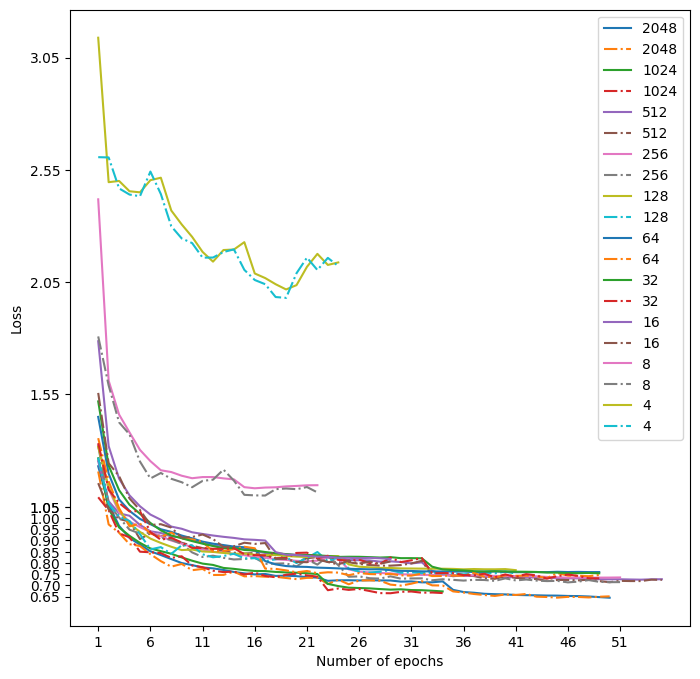
\includegraphics[width=400pt,height=350pt]{pictures/loss.png}
  \caption{Overview of the validation loss of the models trained with different dimensions. The y-axis represents the loss. The x-axis represents the number of epochs. The solid lines represent the mean training loss after each epoch. The dash dot line represents the mean validation loss after each epoch. The numbers in the legend represent the dimension of the latent space representations of the models. }
  \label{fig:loss}
\end{figure} 
 
\subsubsection{Evaluation of the Number of Semantic Subgroups}
\label{sec:conclu_pointnet_semantic}
Once the number of dimensions of the latent space representations is set to 512, next the optimum number of semantic subgroups is evaluated. Since the dataset consists of a large variety of objects, it is not possible to determine a fixed number of categories the objects are to be partitioned into. Thus, the evaluation of the number of subcategories is essential so that the ultimate goal of achieving a set of representative members of the dataset which generalizes the entire dataset quite well is achieved. 

\begin{table}[H]
  \setlength\extrarowheight{10pt}
  \caption{Results of the ConClu approach with PointNet autoencoder on 1000 datapoints when the dimension of the latent space representations is 512 and the number of semantic subgroups is 32. }
  \centering
  \begin{tabular}{|p{30pt}|p{50pt}|p{60pt}|p{50pt}|p{50pt}|p{50pt}|p{40pt}|}
    \toprule
    \ac{t-SNE} dim	& \ac{t-SNE} time & Clustering Algorithm & No. of Clusters & Clustering Time (seconds) & \ac{DBCV} score & \ac{DBCV} Time (seconds)\\
    \midrule
    \multirow{4}{30pt}{2}	& 3.555 & \ac{HDBSCAN}	& 279	& 0.620 & 0.185	& 689.203 \\ \cline{2-7} 
    & 3.731 & k-medoids	& 175	& 0.176 & -0.029	& 101.171 \\ \cline{2-7} 
    & 3.349 & Spectral	& 175	& 7.221 & 0.042 	& 100.748 \\ \cline{2-7}
    & 3.663 & Agglomerative	& 175	& 0.031 & -0.007	& 102.203 \\ 
    \bottomrule
  \end{tabular}
  \label{tab:conclu_k_32}
\end{table}

\begin{table}[H]
  \setlength\extrarowheight{10pt}
  \caption{Results of the ConClu approach on 1000 datapoints for multi-level \ac{HDBSCAN} clustering algorithm when the dimension of the latent space representations is 512 and the number of semantic subgroups is 32. }
  \centering
  \begin{tabular}{|l|l|l|l|l|l|}
    \toprule
    Level & Algorithm	& No. of Clusters	& No. of Outliers	& DBCV score	& \ac{DBCV} time (seconds)	\\  
    \midrule
    Level 1 & \ac{HDBSCAN} & 279	& 96	& 0.185	& 689.203 \\ \cline{1-6}
    Level 2 & \ac{HDBSCAN}	& 122	& 51	& 0.043	& 203.029 \\ 
    \bottomrule
  \end{tabular}
  \label{tab:conclu_k_32_levels}
\end{table}

\begin{table}[H]
  \setlength\extrarowheight{10pt}
  \caption{Results of the ConClu approach with PointNet autoencoder on 1000 datapoints when the dimension of the latent space representations is 512 and the number of semantic subgroups is 16. }
  \centering
  \begin{tabular}{|p{30pt}|p{50pt}|p{60pt}|p{50pt}|p{50pt}|p{50pt}|p{40pt}|}
    \toprule
    \ac{t-SNE} dim	& \ac{t-SNE} time & Clustering Algorithm & No. of Clusters & Clustering Time (seconds) & \ac{DBCV} score & \ac{DBCV} Time (seconds)\\
    \midrule
    \multirow{4}{30pt}{2}	& 3.797 & \ac{HDBSCAN}	& 291	& 0.140 & 0.182	& 244.248 \\ \cline{2-7} 
    & 3.557 & k-medoids	& 175	& 0.257 & -0.50	& 100.699 \\ \cline{2-7} 
    & 3.480 & Spectral	& 175	& 6.331 & 0.030	& 103.005 \\ \cline{2-7}
    & 3.731 & Agglomerative	& 175	& 0.033 & -0.007	& 104.203 \\ 
    \bottomrule
  \end{tabular}
  \label{tab:conclu_k_16}
\end{table}
Tab. \ref{tab:conclu_512} on Pg. 58 already shows the performance of the model when the dimensions of the latent space representation is 512 and the number of semantic subgroups is 64. Tab. \ref{tab:conclu_k_32} records the performance of the model when the number of semantic subgroups is set to 32. Tab. \ref{tab:conclu_k_32_levels} shows the performance of the multi-level \ac{HDBSCAN} algorithm on this model. The rest of the parameters for the experiments remains constant throughout this subsection. It is seen that the performance of the model with $k=32$ is comparable to the model with $k=64$. The \ac{DBCV} score for the model with $k=32$ is 0.185 while that of the model with $k=64$ is 0.186. In other words, even with fewer semantic subgroups the model could achieve comparable results. Moreover, the model for $k=32$ requires a training time of 28 hours for 39 epochs. Whereas, the model for $k=64$ requires a training time of 64 hours for 54 epochs. Thus, reducing the value of k by a factor of 2 also led t the decrease in the training time by a factor of 2.29. This also re-ensures the ultimate goal of the task. Fewer subcategories in the objects means the model will learn more "general" features of the objects and not the extremely intricate and instance-specific object features. This would help in objects of the dataset which actually capture the overall variance in the dataset. Tab. \ref{tab:conclu_k_16} and Tab. \ref{tab:conclu_k_8} shows the performance of the model when the dimension of the latent space representation is 512 and the number of semantic subgroups is 16 and 8 respectively.  Tab. \ref{tab:conclu_k_16_levels} records the performance of multi-level \ac{HDBSCAN} algorithm when the number of semantic subgroups is set to 16. The dimension of the latent space representations of all these models are 512. a batch size of 128 is used to train the models as mentioned earlier. The model for $k=16$ requires a training time of 37 hours for 63 epochs until convergence. Whereas, the model for $k=8$ requires a training time of 31 hours for 40 epochs. It is seen that the model with $k=16$ gives almost comparable results to that of the model with $k=32$. But it is observed that the model with $k=16$ takes longer training time for convergence as compared to the model with $k=32$. It is further noted that the performance of the model with $k=8$ degrades by a factor of 4.3\% as compared to that of the model with $k=8$.

\begin{table}[H]
  \setlength\extrarowheight{10pt}
  \caption{Results of the ConClu approach on 1000 datapoints for multi-level \ac{HDBSCAN} clustering algorithm when the dimension of the latent space representations is 512 and the number of semantic subgroups is 16. }
  \centering
  \begin{tabular}{|l|l|l|l|l|l|}
    \toprule
    Level & Algorithm	& No. of Clusters	& No. of Outliers	& DBCV score	& \ac{DBCV} time (seconds)	\\  
    \midrule
    Level 1 & \ac{HDBSCAN} & 291	& 110	& 0.182	& 244.248 \\ \cline{1-6}
    Level 2 & \ac{HDBSCAN}	& 117	& 38	& 0.033	& 57.618
    \\ 
    \bottomrule
  \end{tabular}
  \label{tab:conclu_k_16_levels}
\end{table}

\begin{table}[H]
  \setlength\extrarowheight{10pt}
  \caption{Results of the ConClu approach with PointNet autoencoder on 1000 datapoints when the dimension of the latent space representations is 512 and the number of semantic subgroups is 8. }
  \centering
  \begin{tabular}{|p{30pt}|p{50pt}|p{60pt}|p{50pt}|p{50pt}|p{50pt}|p{40pt}|}
    \toprule
    \ac{t-SNE} dim	& \ac{t-SNE} time & Clustering Algorithm & No. of Clusters & Clustering Time (seconds) & \ac{DBCV} score & \ac{DBCV} Time (seconds)\\
    \midrule
    \multirow{4}{30pt}{2}	& 3.018 & \ac{HDBSCAN}	& 291	& 0.140 & 0.139 	& 235.023 \\ \cline{2-7} 
    & 3.091 & k-medoids	& 175	& 0.191 & -0.092	& 98.415 \\ \cline{2-7} 
    & 3.101 & Spectral	& 175	& 6.810 & -0.027	& 96.898 \\ \cline{2-7}
    & 3.177 & Agglomerative	& 175	& 0.038 & -0.030	& 97.490 \\ 
    \bottomrule
  \end{tabular}
  \label{tab:conclu_k_8}
\end{table}

\begin{table}[H]
  \setlength\extrarowheight{10pt}
  \caption{Results of the ConClu approach with PointNet autoencoder on 1000 datapoints when the dimension of the latent space representations is 512 and the number of semantic subgroups is 128. }
  \centering
  \begin{tabular}{|p{30pt}|p{50pt}|p{60pt}|p{50pt}|p{50pt}|p{50pt}|p{40pt}|}
    \toprule
    \ac{t-SNE} dim	& \ac{t-SNE} time & Clustering Algorithm & No. of Clusters & Clustering Time (seconds) & \ac{DBCV} score & \ac{DBCV} Time (seconds)\\
    \midrule
    \multirow{4}{30pt}{2}	& 3.259 & \ac{HDBSCAN}	& 301	& 0.115 & 0.186 	& 332.309 \\ \cline{2-7} 
    & 4.356 & k-medoids	& 175	& 0.172 & -0.049	& 205.339 \\ \cline{2-7} 
    & 3.344 & Spectral	& 175	& 11.716 & 0.024	& 166.501 \\ \cline{2-7}
    & 5.815 & Agglomerative	& 175	& 0.049 & -0.041	& 170.280 \\ 
    \bottomrule
  \end{tabular}
  \label{tab:conclu_k_128}
\end{table} 

\begin{table}[H]
  \setlength\extrarowheight{10pt}
  \caption{Results of the ConClu approach with PointNet autoencoder on 1000 datapoints when the dimension of the latent space representations is 512 and the number of semantic subgroups is 4. }
  \centering
  \begin{tabular}{|p{30pt}|p{50pt}|p{60pt}|p{50pt}|p{50pt}|p{50pt}|p{40pt}|}
    \toprule
    \ac{t-SNE} dim	& \ac{t-SNE} time & Clustering Algorithm & No. of Clusters & Clustering Time (seconds) & \ac{DBCV} score & \ac{DBCV} Time (seconds)\\
    \midrule
    \multirow{4}{30pt}{2}	& 3.295 & \ac{HDBSCAN}	& 296	& 0.122 & 0.103	& 269.228 \\ \cline{2-7} 
    & 3.577 & k-medoids	& 175	& 0.308 & -0.045	& 139.550 \\ \cline{2-7} 
    & 3.751 & Spectral	& 175	& 11.623 & -0.004	& 167.611 \\ \cline{2-7}
    & 5.013 & Agglomerative	& 175	& 0.032 & -0.005	& 169.509 \\ 
    \bottomrule
  \end{tabular}
  \label{tab:conclu_k_4}
\end{table} 

\begin{table}[H]
  \setlength\extrarowheight{10pt}
  \caption{Results of the ConClu approach with PointNet autoencoder on 1000 datapoints when the dimension of the latent space representations is 512 and the number of semantic subgroups is 2. }
  \centering
  \begin{tabular}{|p{30pt}|p{50pt}|p{60pt}|p{50pt}|p{50pt}|p{50pt}|p{40pt}|}
    \toprule
    \ac{t-SNE} dim	& \ac{t-SNE} time & Clustering Algorithm & No. of Clusters & Clustering Time (seconds) & \ac{DBCV} score & \ac{DBCV} Time (seconds)\\
    \midrule
    \multirow{4}{30pt}{2}	& 4.469 & \ac{HDBSCAN}	& 289	& 0.126 & 0.085	& 320.217 \\ \cline{2-7} 
    & 3.364 & k-medoids	& 175	& 5.662 & -0.118 	& 155.136 \\ \cline{2-7} 
    & 3.349 & Spectral	& 175	& 5.662 & -0.089	& 115.978 \\ \cline{2-7}
    & 3.029 & Agglomerative	& 175	& 0.038 & -0.100	& 98.683 \\ 
    \bottomrule
  \end{tabular}
  \label{tab:conclu_k_2}
\end{table}

Tab. \ref{tab:conclu_k_128} shows the performance of the model when the dimension of the latent space representation is 512 and the number of semantic subgroups is 128. The model requires a training time of 58 hours for 36 epochs until convergence is reached.

\begin{figure}[H]
  \centering
  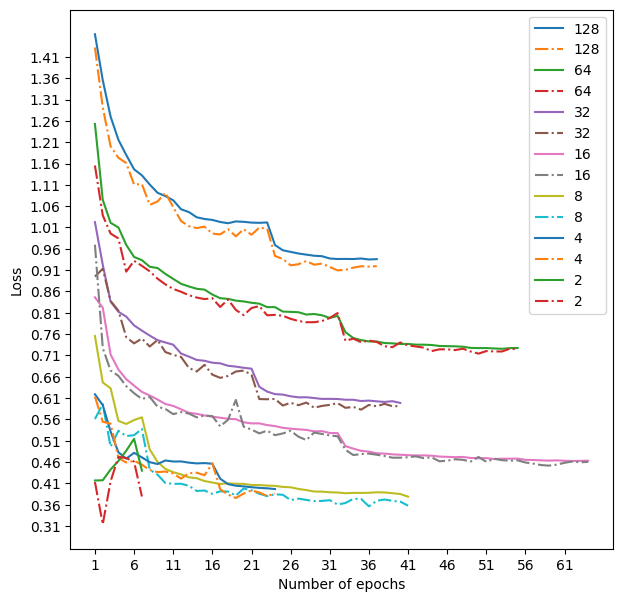
\includegraphics[width=400pt,height=300pt]{pictures/loss_k.png}
  \caption{Overview of the validation loss of the models trained with different values of semantic subgroups when dimension of the latent space representation is fixed to 512. The y-axis represents the loss. The x-axis represents the number of epochs. The solid lines represent the mean training loss after each epoch. The dash dot line represents the mean validation loss after each epoch. The numbers in the legend represent number of semantic subgroups in the objects.}
  \label{fig:loss_k}
\end{figure} 

It can be seen that the performance for the model with $k=128$ is comparable to the model with $k=32$. Also, the training time for the model with $k=32$ is much less compared to that of the model with $k=128$. Tab. \ref{tab:conclu_k_4} and Tab. \ref{tab:conclu_k_2} shows the performance of the model when the dimension of the latent space representation is 512 and the number of semantic subgroups is 4 and 2 respectively. The training time for the model with $k=4$ is 17 hours for 23 epochs. Similarly, the training time for the model with $k=2$ is 5 hours for 6 epochs. It can be observed that the performance of the models decline significantly when the number of semantic subgroups is too low. Thus, it can be concluded that the performance of the models increases with the increase in the number of semantic subgroups and then attains a saturation in the performance. In other words, the number of semantic subgroups doesn't effect the performance of the models as long as they are enough parts the objects are partitioned into. Tab. \ref{tab:conclu_k_128} shows the performance of the model when the dimension of the latent space representation is 512 and the number of semantic subgroups is 128. The model requires a training time of 58 hours for 36 epochs until convergence is reached. It can be seen that the performance for the model with $k=128$ is comparable to the model with $k=32$. Also, the training time for the model with $k=32$ is much less compared to that of the model with $k=128$. 


\subsubsection{Evaluation of the Batch Size for Training}
One of the most crucial hyperparameters to adjust in deep learning methods is batch size. Attempting to optimize convex functions involves an intrinsic trade-off between the advantages of larger and smaller batch sizes. One way to ensure convergence to the global optima of the objective function is to use a batch size equal to the entire dataset. But doing so comes at the expense of a slower empirical convergence to that optimal state. Also, it practically infeasible to load the entire dataset like the ABC dataset \cite{Koch_2019_CVPR} in this use-case all at once. However, it has been demonstrated empirically that employing lower batch sizes leads to a faster convergence to "good" solutions. Smaller batch sizes enable the model to "start learning before having to see all the data," which provides an easy explanation for this. A smaller batch size has the drawback of not guaranteeing that the model will eventually come to the global optima. It will oscillate between the global optima, remaining outside a certain $\epsilon$-ball of the optima, where $\epsilon$ is determined by the batch size to dataset ratio. Therefore, as mentioned in Ch. \ref{sec:hardware}, the largest batch size that could be fit in the GPU with the higher capacity is observed to be 256. Thus, to facilitate the training of multiple models for experimentation in the limited time frame parallelly, the performance of the models with batch sizes 64, 128 and 256 are evaluated. The dimension of the latent space representations of the all the models in this subsection is set to 512 and $k=32$ as discussed above. The learning rate is 0.001 and the decay factor for the learning rate is 0.1 as mentioned earlier. Tab. \ref{tab:conclu_k_32} on Pg. 63 already shows the performance of the model when batch size is 128. Tab. \ref{tab:conclu_batch_256} shows the performance of the model when the batch size is 256. The training time for this model is 40 hours for 43 epochs. Tab. \ref{tab:conclu_batch_256_levels} records the performance of the multi-level \ac{HDBSCAN} algorithm.
\begin{table}[H]
  \setlength\extrarowheight{10pt}
  \caption{Results of the ConClu approach with PointNet autoencoder on 1000 datapoints when the dimension of the latent space representations is 512, the number of semantic subgroups is 32 and the batch size for training the model is 256. }
  \centering
  \begin{tabular}{|p{30pt}|p{50pt}|p{60pt}|p{50pt}|p{50pt}|p{50pt}|p{40pt}|}
    \toprule
    \ac{t-SNE} dim	& \ac{t-SNE} time & Clustering Algorithm & No. of Clusters & Clustering Time (seconds) & \ac{DBCV} score & \ac{DBCV} Time (seconds)\\
    \midrule
    \multirow{4}{30pt}{2}	& 5.855 & \ac{HDBSCAN}	& 291	& 0.178 & 0.154 & 382.814 \\ \cline{2-7} 
    & 6.034 & k-medoids	& 175	& 0.384 & -0.040	& 146.189 \\ \cline{2-7} 
    & 5.365 & Spectral	& 175	& 13.660 & 0.026	& 145.207 \\ \cline{2-7}
    & 5.513 & Agglomerative	& 175	& 0.040 & -0.011	& 167.093 \\ 
    \bottomrule
  \end{tabular}
  \label{tab:conclu_batch_256}
\end{table}

\begin{table}[H]
  \setlength\extrarowheight{10pt}
  \caption{Results of the ConClu approach on 1000 datapoints for multi-level \ac{HDBSCAN} clustering algorithm when the dimension of the latent space representations is 512, the number of semantic subgroups is 32 and the batch size for training the model is 256. }
  \centering
  \begin{tabular}{|l|l|l|l|l|l|}
    \toprule
    Level & Algorithm	& No. of Clusters	& No. of Outliers	& DBCV score	& \ac{DBCV} time (seconds)	\\  
    \midrule
    Level 1 & \ac{HDBSCAN} & 291	& 92	& 0.154	& 382.814 \\ \cline{1-6}
    Level 2 & \ac{HDBSCAN} & 126	& 53	& 0.038	& 101.948 \\ 
    \bottomrule
  \end{tabular}
  \label{tab:conclu_batch_256_levels}
\end{table}

It is seen that this algorithm gives the second-best clustering results after \ac{HDBSCAN} algorithm. And the result is slightly better than that of spectral clustering. Quite naturally, the model takes longer to converge for a larger batch size. But performance of the model does not seem to improve as expected as compared to the model with batch size 128. The \ac{DBCV} of the \ac{HDBSCAN} algorithm is 0.185 for the earlier model, whereas for the model with batch size it appears to suffer a downfall in performance by 3.1\%.

\begin{table}[H]
  \setlength\extrarowheight{10pt}
  \caption{Results of the ConClu approach with PointNet autoencoder on 1000 datapoints when the dimension of the latent space representations is 512, the number of semantic subgroups is 32 and the batch size for training the model is 64. }
  \centering
  \begin{tabular}{|p{30pt}|p{50pt}|p{60pt}|p{50pt}|p{50pt}|p{50pt}|p{40pt}|}
    \toprule
    \ac{t-SNE} dim	& \ac{t-SNE} time & Clustering Algorithm & No. of Clusters & Clustering Time (seconds) & \ac{DBCV} score & \ac{DBCV} Time (seconds)\\
    \midrule
    \multirow{4}{30pt}{2}	& 5.454 & \ac{HDBSCAN}	& 300	& 1.080 & 0.177	& 730.026 \\ \cline{2-7} 
    & 6.732 & k-medoids	& 175	& 7.606 & -0.056	& 602.923 \\ \cline{2-7} 
    & 6.326 & Spectral	& 175	& 51.657 & 0.008	& 492.017 \\ \cline{2-7}
    & 6.129 & Agglomerative	& 175	& 0.489 & -0.007 &	481.838 \\ 
    \bottomrule
  \end{tabular}
  \label{tab:conclu_batch_64}
\end{table}

\begin{table}[H]
  \setlength\extrarowheight{10pt}
  \caption{Results of the ConClu approach on 1000 datapoints for multi-level \ac{HDBSCAN} clustering algorithm when the batch size for training the model is 64. }
  \centering
  \begin{tabular}{|l|l|l|l|l|l|}
    \toprule
    Level & Algorithm	& No. of Clusters	& No. of Outliers	& DBCV score	& \ac{DBCV} time (seconds)	\\  
    \midrule
    Level 1 & \ac{HDBSCAN} & 300	& 85	& 0.177	& 730.026 \\ \cline{1-6}
    Level 2 & \ac{HDBSCAN} & 128	& 41	& 0.035	& 210.596 \\ 
    \bottomrule
  \end{tabular}
  \label{tab:conclu_batch_64_levels}
\end{table}

\begin{figure}[H]
  \centering
  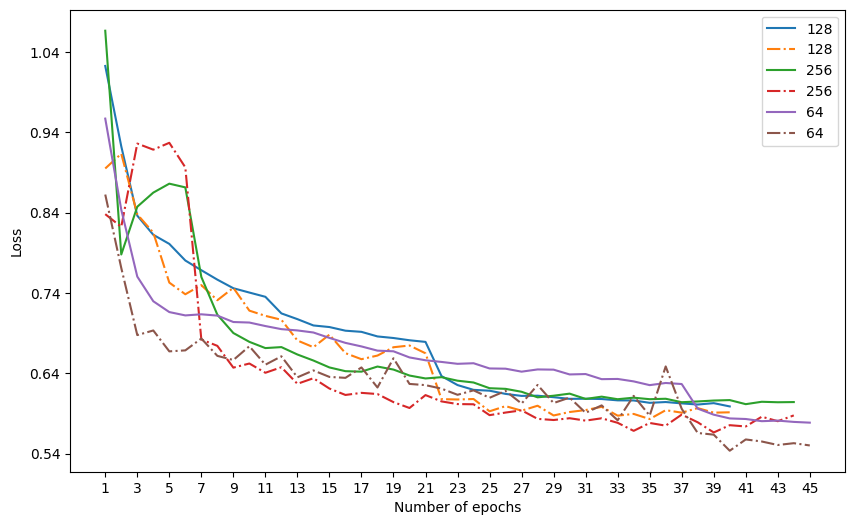
\includegraphics[width=400pt,height=200pt]{pictures/loss_batch.png}
  \caption{Overview of the validation loss of the models trained with different batch sizes when dimension of the latent space representation is fixed to 512 and the number of semantic subgroups to 32. The y-axis represents the loss. The x-axis represents the number of epochs. The solid lines represent the mean training loss after each epoch. The dash dot line represents the mean validation loss after each epoch. The numbers in the legend represent the batch size used for training the models. }
  \label{fig:loss_batch}
\end{figure} 

On the other hand, Tab. \ref{tab:conclu_batch_64} shows the performance of the model when the batch size is 64. Tab. \ref{tab:conclu_batch_64_levels} documents the performance of the multi-level \ac{HDBSCAN} algorithm on this model. The training time for this model is 36 hours for 44 epochs. The performance of the models is seen to improve from batch size 64 to 128 as expected. Fig. \ref{fig:loss_batch} gives an overview of the training and validation loss of the models with changing batch size. It can be observed that the validation loss of the models are quite comparable on convergence which can justify the reason behind no significant improvement of the models with different batch sizes. 

\subsubsection{Evaluation of the Effect of Early Stopping}
Determining an appropriate finite number of training epochs is a major challenge while developing machine learning models. If a model has too less epochs, then it would result to an underfit model whereas if the number of epochs is too large, then the model tends to memorize the training dataset and doesn't generalize well for unseen data \cite{Goodfellow-et-al-2016}. Therefore, the method of termination of the training when the model no longer improves its performance on the validation dataset is known as the early stopping mechanism. The patience parameter plays a very vital role in this mechanism. The model does not immediately terminate the training as soon as there is an increase in the validation loss. Rather it waits for a number of consecutive epochs defined by the patience parameter. And if the validation loss no longer decreases as compared to the least recorded validation loss, the training is then terminated.

\begin{table}[H]
  \setlength\extrarowheight{10pt}
  \caption{Results of the ConClu approach with PointNet autoencoder on 1000 datapoints when the patience for early stopping is 3, dimension of the latent space representations is 512, the number of semantic subgroups is 32 and the batch size for training the model is 128. }
  \centering
  \begin{tabular}{|p{30pt}|p{50pt}|p{60pt}|p{50pt}|p{50pt}|p{50pt}|p{40pt}|}
    \toprule
    \ac{t-SNE} dim	& \ac{t-SNE} time & Clustering Algorithm & No. of Clusters & Clustering Time (seconds) & \ac{DBCV} score & \ac{DBCV} Time (seconds)\\
    \midrule
    \multirow{4}{30pt}{2}	& 3.643 & \ac{HDBSCAN}	& 289	& 0.112 & 0.132	& 260.046 \\ \cline{2-7} 
    & 3.614 & k-medoids	& 175	& 0.101	& -0.054	& 115.333 \\ \cline{2-7} 
    & 3.535 & Spectral	& 175	& 5.567	& -0.008	& 114.561 \\ \cline{2-7}
    & 3.765 & Agglomerative	& 175	& 0.299	& -0.033	& 106.243 \\ 
    \bottomrule
  \end{tabular}
  \label{tab:conclu_patience_3}
\end{table}

\begin{table}[H]
  \setlength\extrarowheight{10pt}
  \caption{Results of the ConClu approach on 1000 datapoints for multi-level \ac{HDBSCAN} clustering algorithm when the patience for early stopping is 3. }
  \centering
  \begin{tabular}{|l|l|l|l|l|l|}
    \toprule
    Level & Algorithm	& No. of Clusters	& No. of Outliers	& DBCV score	& \ac{DBCV} time (seconds)	\\  
    \midrule
    Level 1 & \ac{HDBSCAN} & 289	& 98	& 0.132	& 260.046 \\ \cline{1-6}
    Level 2 & \ac{HDBSCAN} & 119	& 41	& -0.003	& 63.805 \\ 
    \bottomrule
  \end{tabular}
  \label{tab:conclu_patience_3_levels}
\end{table}
A patience of 3, 5, 7 and 10 have been evaluated in this subsection. The learning rate of 0.001 and a decay factor of 0.1 as mentioned earlier is used throughout the experiments recorded below. Tab. \ref{tab:conclu_patience_3} shows the performance of the model with patience 3. Tab. \ref{tab:conclu_patience_3_levels} records the performance of multi-level \ac{HDBSCAN} algorithm on this model. The model takes a training time of 10 hours for 10 epochs until convergence. Tab. \ref{tab:conclu_k_32} on Pg. 63 already shows the performance of the model when the patience parameter is set to 5. It requires a training time of 28 hours for 39 epochs. As expected the model with less patience has lower training time compared to that with a high patience. But it is that the performance of the model with less patience is worse as compared to that with higher patience. There is a 5\% decline in the quality of the performance. 

\begin{table}[H]
  \setlength\extrarowheight{10pt}
  \caption{Results of the ConClu approach with PointNet autoencoder on 1000 datapoints when the patience for early stopping is 7, dimension of the latent space representations is 512, the number of semantic subgroups is 32 and the batch size for training the model is 128. }
  \centering
  \begin{tabular}{|p{30pt}|p{50pt}|p{60pt}|p{50pt}|p{50pt}|p{50pt}|p{40pt}|}
    \toprule
    \ac{t-SNE} dim	& \ac{t-SNE} time & Clustering Algorithm & No. of Clusters & Clustering Time (seconds) & \ac{DBCV} score & \ac{DBCV} Time (seconds)\\
    \midrule
    \multirow{4}{30pt}{2}	& 3.731	& \ac{HDBSCAN}	& 298	& 0.126	& 0.199	& 293.794
    \\ \cline{2-7} 
    & 3.257	& k-medoids	& 175	& 0.134	& -0.037	& 116 \\ \cline{2-7} 
    & 3.340	& Spectral	& 175	& 9.391	& 0.011	& 94.393 \\ \cline{2-7}
    & 2.788	& Agglomerative	& 175	& 0.032	& -0.018	& 93.149 \\ 
    \bottomrule
  \end{tabular}
  \label{tab:conclu_patience_7}
\end{table}

\begin{table}[H]
  \setlength\extrarowheight{10pt}
  \caption{Results of the ConClu approach on 1000 datapoints for multi-level \ac{HDBSCAN} clustering algorithm when the patience for early stopping is 7. }
  \centering
  \begin{tabular}{|l|l|l|l|l|l|}
    \toprule
    Level & Algorithm	& No. of Clusters	& No. of Outliers	& DBCV score	& \ac{DBCV} time (seconds)	\\  
    \midrule
    Level 1 & \ac{HDBSCAN} & 298	& 99	& 0.199	& 293.794 \\ \cline{1-6}
    Level 2 & \ac{HDBSCAN} & 117	& 40	& 0.013	& 64.412
    \\ 
    \bottomrule
  \end{tabular}
  \label{tab:conclu_patience_7_levels}
\end{table}

\begin{table}[H]
  \setlength\extrarowheight{10pt}
  \caption{Results of the ConClu approach with PointNet autoencoder on 1000 datapoints when the patience for early stopping is 10, dimension of the latent space representations is 512, the number of semantic subgroups is 32 and the batch size for training the model is 128. }
  \centering
  \begin{tabular}{|p{30pt}|p{50pt}|p{60pt}|p{50pt}|p{50pt}|p{50pt}|p{40pt}|}
    \toprule
    \ac{t-SNE} dim	& \ac{t-SNE} time & Clustering Algorithm & No. of Clusters & Clustering Time (seconds) & \ac{DBCV} score & \ac{DBCV} Time (seconds)\\
    \midrule
    \multirow{4}{30pt}{2}	& 3.338	& \ac{HDBSCAN}	& 308	& 0.126	& 0.190	& 330.257 \\ \cline{2-7} 
    & 3.191	& k-medoids	& 175	& 0.288	& -0.051	& 166.315 \\ \cline{2-7} 
    & 3.072	& Spectral	& 175	& 7.785	& 0.013	& 156.930 \\ \cline{2-7}
    & 3.441	& Agglomerative	& 175	& 0.032	& -0.041	& 159.887 \\ 
    \bottomrule
  \end{tabular}
  \label{tab:conclu_patience_10}
\end{table}

Tab. \ref{tab:conclu_patience_7} and Tab. \ref{tab:conclu_patience_10} shows the performance of the models with patience 7 and 10 respectively. The former model takes a training time of 46 hours for 49 epochs. As expected, the model takes more number of epochs until convergence as compared to the model with patience 5. Also, the results for this model outperform the performance shown by the model with patience 3 and 5 as expected. Tab. \ref{tab:conclu_patience_7_levels} shows the performance of multi-level \ac{HDBSCAN} algorithm on this model. The \ac{DBCV} score attained by the \ac{HDBSCAN} algorithm is 0.199 by this model as coma
pared to the next best model with patience 5 which has the \ac{DBCV} score of 0.185. The model with patience 10 requires a training time of 30 hours for 42 epochs. But the performance of the model is seen to drop a bit as compared to the model with patience 7. Fig. \ref{fig:loss_early_stopping_patience} gives an overview of the training and validation loss of the models for different values of the patience parameter. As expected, the model with patience 10 has the least validation loss on convergence. Thus, weighing the training time of the models and their performance for the clustering task, the model with patience 7 is observed to have the best results. 

\begin{figure}[H]
  \centering
  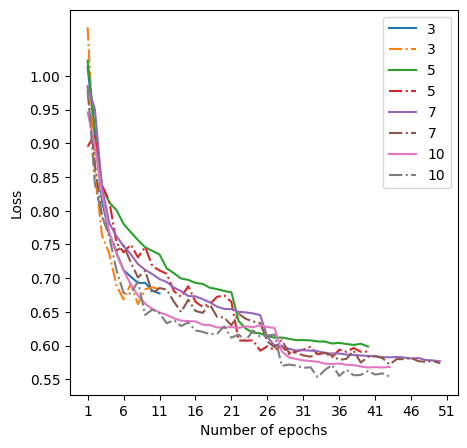
\includegraphics[width=350pt,height=250pt]{pictures/loss_early_stopping_patience.png}
  \caption{Overview of the validation loss of the models trained with different values of the patience parameter in early stopping when dimension of the latent space representation is fixed to 512, the number of semantic subgroups is 32 and batch size is 128. The y-axis represents the loss. The x-axis represents the number of epochs. The solid lines represent the mean training loss after each epoch. The dash dot line represents the mean validation loss after each epoch. The numbers in the legend represent the value of the patience parameter. }
  \label{fig:loss_early_stopping_patience}
\end{figure} 

\subsubsection{Evaluation of the Effect of Learning Rate}
The learning rate is one of the crucial hyperparameters when building a machine learning model. When the model weights are updated, it regulates how much the model is to be altered after calculating the estimated error. Carefully selecting the learning rate is extremely necessary because if the learning rate is too small, then the training process will be extremely low and it can get stuck at a local minima. Whereas, if the learning rate s too high, then the model can oscillate around the global optima without reaching a convergence. Tab. \ref{tab:conclu_32} on Pg. 60 already shows the performance of the model when the learning rate is set to 0.001. Tab. \ref{tab:conclu_lr_01} documents the performance of the model when the learning rate is set to 0.01. The model requires a training time of 28 hours for 40 epochs. It takes almost the same number of epochs to converge as does the model with learning rate 0.001. Furthermore, it can be observed that the performance of the model deteriorates when the learning rate is changed to 0.01 from 0.001. There is a 6\% degradation in performance when the learning rate is increased by a factor of 10. Tab. \ref{tab:conclu_lr_01_levels} shows the performance of the multi-level \ac{HDBSCAN} algorithm on this model.
\begin{table}[H]
  \setlength\extrarowheight{10pt}
  \caption{Results of the ConClu approach with PointNet autoencoder on 1000 datapoints when the learning rate is 0.01. }
  \centering
  \begin{tabular}{|p{30pt}|p{50pt}|p{60pt}|p{50pt}|p{50pt}|p{50pt}|p{40pt}|}
    \toprule
    \ac{t-SNE} dim	& \ac{t-SNE} time & Clustering Algorithm & No. of Clusters & Clustering Time (seconds) & \ac{DBCV} score & \ac{DBCV} Time (seconds)\\
    \midrule
    \multirow{4}{30pt}{2}	& 3.417	& \ac{HDBSCAN}	& 285	& 0.109	& 0.128	& 315.829 \\ \cline{2-7} 
    & 3.455	& k-medoids	& 175	& 0.246	& -0.038	& 147.585 \\ \cline{2-7} 
    & 3.270	& Spectral	& 175	& 6.347	& -0.057	& 156.651 \\ \cline{2-7}
    & 3.844	& Agglomerative	& 175	& 0.037	& -0.083	& 162.778 \\ 
    \bottomrule
  \end{tabular}
  \label{tab:conclu_lr_01}
\end{table} 

\begin{table}[H]
  \setlength\extrarowheight{10pt}
  \caption{Results of the ConClu approach on 1000 datapoints for multi-level \ac{HDBSCAN} clustering algorithm when the learning rate is 0.01. }
  \centering
  \begin{tabular}{|l|l|l|l|l|l|}
    \toprule
    Level & Algorithm	& No. of Clusters	& No. of Outliers	& DBCV score	& \ac{DBCV} time (seconds)	\\  
    \midrule
    Level 1 & \ac{HDBSCAN} & 285	& 107	& 0.128	& 315.829 \\ \cline{1-6}
    Level 2 & \ac{HDBSCAN} & 121	& 42	& -0.049	& 62.360 \\ 
    \bottomrule
  \end{tabular}
  \label{tab:conclu_lr_01_levels}
\end{table}

\subsubsection{Evaluation of the Effect of Decay Factor of the Learning Rate}

Keeping the learning rate and the rest of the parameters constant, experiments are performed to evaluate the effect of the decay factor of the learning rate on the performance of the model. The decay factor determines the value of the new learning rate as shown in Eq. \ref{eq:lr_decay} when the metrices for the performance of the model stops improving.

\begin{equation}
  \label{eq:lr_decay}
  new \; learning \; rate = decay \; factor \times current \; learning \; rate
\end{equation}

Tab. \ref{tab:conclu_32} on Pg. 60 already shows the performance of the model when the learning rate is set to 0.001 and the decay factor is 0.1. Tab. \ref{tab:conclu_lr_decay_5} shows the performance of the model when the learning rate remains constant at 0.001 but the decay factor is change to 0.5. Tab. \ref{tab:conclu_lr_decay_5_levels} shows the performance of multi-level \Ac{HDBSCAN} algorithm on this model. The performance of this model is seen to improve as compared to model with decay factor 0.1. There is almost a 3\% increase in the performance of the model. The decay factor is further increased and Tab. \ref{tab:conclu_lr_decay_9} records the performance of the model when the decay factor is 0.9. All the remaining parameters of the model remains constant. The model takes a training time of 20 hours for 26 epochs until convergence. A decrease in performance of the model is observed as compared to the model with decay rate 0.5.

\begin{table}[H]
  \setlength\extrarowheight{10pt}
  \caption{Results of the ConClu approach with PointNet autoencoder on 1000 datapoints when the learning rate is 0.001 and the decay factor is 0.5. }
  \centering
  \begin{tabular}{|p{30pt}|p{50pt}|p{60pt}|p{50pt}|p{50pt}|p{50pt}|p{40pt}|}
    \toprule
    \ac{t-SNE} dim	& \ac{t-SNE} time & Clustering Algorithm & No. of Clusters & Clustering Time (seconds) & \ac{DBCV} score & \ac{DBCV} Time (seconds)\\
    \midrule
    \multirow{4}{30pt}{2}	& 3.351	& \ac{HDBSCAN}	& 303	& 0.113	& 0.212	& 334.613 \\ \cline{2-7} 
    & 3.734	& k-medoids	& 175	& 0.273	& -0.033	& 164.001 \\ \cline{2-7} 
    & 3.192	& Spectral	& 175	& 6.865	& 0.003	& 109.385 \\ \cline{2-7}
    & 3.722	& Agglomerative	& 175	& 0.043	& -0.001	& 92.632 \\ 
    \bottomrule
  \end{tabular}
  \label{tab:conclu_lr_decay_5}
\end{table}

\begin{table}[H]
  \setlength\extrarowheight{10pt}
  \caption{Results of the ConClu approach on 1000 datapoints for multi-level \ac{HDBSCAN} clustering algorithm when the learning rate is 0.001 and the decay factor is 0.5. }
  \centering
  \begin{tabular}{|l|l|l|l|l|l|}
    \toprule
    Level & Algorithm	& No. of Clusters	& No. of Outliers	& DBCV score	& \ac{DBCV} time (seconds)	\\  
    \midrule
    Level 1 & \ac{HDBSCAN} & 303	& 71	& 0.212	& 334.613 \\ \cline{1-6}
    Level 2 & \ac{HDBSCAN} & 118	& 34	& 0.009	& 62.142 \\ 
    \bottomrule
  \end{tabular}
  \label{tab:conclu_lr_decay_5_levels}
\end{table}

\begin{table}[H]
  \setlength\extrarowheight{10pt}
  \caption{Results of the ConClu approach with PointNet autoencoder on 1000 datapoints when the learning rat is 0.001 and the decay factor is 0.9. }
  \centering
  \begin{tabular}{|p{30pt}|p{50pt}|p{60pt}|p{50pt}|p{50pt}|p{50pt}|p{40pt}|}
    \toprule
    \ac{t-SNE} dim	& \ac{t-SNE} time & Clustering Algorithm & No. of Clusters & Clustering Time (seconds) & \ac{DBCV} score & \ac{DBCV} Time (seconds)\\
    \midrule
    \multirow{4}{30pt}{2}	& 3.265	& \ac{HDBSCAN}	& 287	& 0.114	& 0.184	& 225.236 \\ \cline{2-7} 
    & 3.298	& k-medoids	& 175	& 0.144	& 0.010	& 95.764 \\ \cline{2-7} 
    & 4.107	& Spectral	& 175	& 14.298	& 0.036	& 116.901 \\ \cline{2-7}
    & 3.297	& Agglomerative	& 175	& 0.033	& 0.017	& 96.614 \\ 
    \bottomrule
  \end{tabular}
  \label{tab:conclu_lr_decay_9}
\end{table}

Fig. \ref{fig:loss_lr} gives an overview of the training and validation loss of the models for learning rate and decay factor of the learning rate used during training the models. Even with a lower higher learning rate, the model takes almost the same number of epoch until convergence. But it can be noticed that the model reaches a comparable validation loss quite early on as compared to the model with a lower learning rate. The model with learning rate  0.001 as decay factor 0.9 takes the least training time. 

\begin{table}[H]
  \setlength\extrarowheight{10pt}
  \caption{Results of the ConClu approach on 1000 datapoints for multi-level \ac{HDBSCAN} clustering algorithm when the learning rate is 0.001 and the decay factor is 0.9. }
  \centering
  \begin{tabular}{|l|l|l|l|l|l|}
    \toprule
    Level & Algorithm	& No. of Clusters	& No. of Outliers	& DBCV score	& \ac{DBCV} time (seconds)	\\  
    \midrule
    Level 1 & \ac{HDBSCAN} & 287	& 80	& 0.184	& 225.236 \\ \cline{1-6}
    Level 2 & \ac{HDBSCAN} & 120	& 46	& 0.044	& 56.283 \\ 
    \bottomrule
  \end{tabular}
  \label{tab:conclu_lr_decay_9_levels}
\end{table}

\begin{figure}[H]
  \centering
  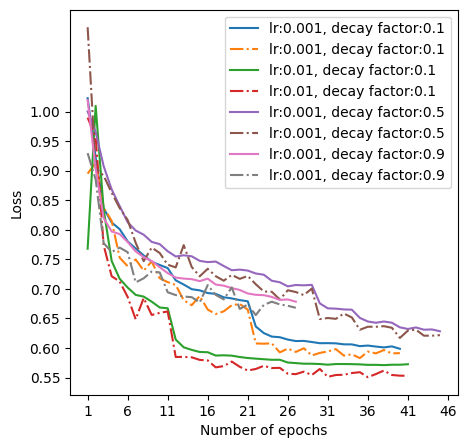
\includegraphics[width=300pt,height=280pt]{pictures/loss_lr.png}
  \caption{Overview of the validation loss of the models trained with different values of learning rate and decay factor of the learning rate when dimension of the latent space representation is fixed to 512, the number of semantic subgroups is 32 and batch size is 128. The y-axis represents the loss. The x-axis represents the number of epochs. The solid lines represent the mean training loss after each epoch. The dash dot line represents the mean validation loss after each epoch. The numbers in the legend represent the learning rate and decay factor of the learning rate.}
  \label{fig:loss_lr}
\end{figure} 

\subsection{ConClu Approach with Dynamic Graph Convolutional Neural Network as Backbone}
\label{sec:conclu_dgcnn}

As mentioned in Ch. \ref{sec:method}, two feature representation learning backbones are used for the experiments. Experiments with the \ac{DGCNN} as the backbone is recorded here. The performance of all the clustering algorithms are evaluated.

\subsubsection{Evaluation of dimension of feature space representations}
As discussed earlier, the dimension of the latent space representation is an extremely crucial parameter while training the network. Since the original dataset has the point clouds with 2048 points in each of them, for the sake of completeness of the experimentation, the evaluation are performed for all dimensions on a logarithmic scale of 2 from 1024 to down until 4. Tab. \ref{tab:dgcnn_1024} shows the experiments when the dimension of the latent space representations is set to be 1024. Tab. \ref{tab:dgcnn_1024_levels} shows the performance of multi-level \ac{HDBSCAN} model on this model. For all the models in this subsection, the number of nearest neighbors requires for a \ac{DGCNN} graph is set to 20 based on \cite{mei2022unsupervised}.

\begin{table}[H]
  \setlength\extrarowheight{10pt}
  \caption{Results of the ConClu approach with \ac{DGCNN} backbone on 1000 datapoints when the dimension of the latent space representation is 1024. }
  \centering
  \begin{tabular}{|p{30pt}|p{50pt}|p{60pt}|p{50pt}|p{50pt}|p{50pt}|p{40pt}|}
    \toprule
    \ac{t-SNE} dim	& \ac{t-SNE} time & Clustering Algorithm & No. of Clusters & Clustering Time (seconds) & \ac{DBCV} score & \ac{DBCV} Time (seconds)\\
    \midrule
    \multirow{4}{30pt}{2}	& 3.022	& \ac{HDBSCAN}	& 295	& 0.121 & 0.112	& 228.925 \\ \cline{2-7} 
    & 3.519 & k-medoids	& 175	& 0.151 & -0.067	& 92.043 \\ \cline{2-7} 
    & 3.212 & Spectral	& 175	& 6.712 & -0.038 	& 92.080 \\ \cline{2-7}
    & 3.683 & Agglomerative	& 175	& 0.037 & -0.089	& 124.850 \\ 
    \bottomrule
  \end{tabular}
  \label{tab:dgcnn_1024}
\end{table}

\begin{table}[H]
  \setlength\extrarowheight{10pt}
  \caption{Results of the ConClu approach on 1000 datapoints for multi-level \ac{HDBSCAN} clustering algorithm when the dimension of the latent space representation is 1024. }
  \centering
  \begin{tabular}{|l|l|l|l|l|l|}
    \toprule
    Level & Algorithm	& No. of Clusters	& No. of Outliers	& DBCV score	& \ac{DBCV} time (seconds)	\\  
    \midrule
    Level 1 & \ac{HDBSCAN} & 295	& 89	& 0.112	& 228.925  \\ \cline{1-6}
    Level 2 & \ac{HDBSCAN} & 132	& 40	& -0.035	& 86.639 \\ 
    \bottomrule
  \end{tabular}
  \label{tab:dgcnn_1024_levels}
\end{table}

\begin{table}[H]
  \setlength\extrarowheight{10pt}
  \caption{Results of the ConClu approach with \ac{DGCNN} backbone on 1000 datapoints when the dimension of the latent space representation is 512. }
  \centering
  \begin{tabular}{|p{30pt}|p{50pt}|p{60pt}|p{50pt}|p{50pt}|p{50pt}|p{40pt}|}
    \toprule
    \ac{t-SNE} dim	& \ac{t-SNE} time & Clustering Algorithm & No. of Clusters & Clustering Time (seconds) & \ac{DBCV} score & \ac{DBCV} Time (seconds)\\
    \midrule
    \multirow{4}{30pt}{2}	& 3.214 & \ac{HDBSCAN}	& 299	& 0.125 & 0.129	& 327.926 \\ \cline{2-7} 
    & 3.739 & k-medoids	& 175	& 0.248 & -0.060	& 162.210 \\ \cline{2-7} 
    & 3.212 & Spectral	& 175	& 6.712 & -0.038 & 92.080 \\ \cline{2-7}
    & 3.683 & Agglomerative	& 175	& 0.037 & -0.089	& 124.850 \\ 
    \bottomrule
  \end{tabular}
  \label{tab:dgcnn_512}
\end{table}

It is observed that training the models with the \ac{DGCNN} backbone takes extremely large training time. The model with the dimension of latent space representation of 1024 takes 168 hours for 37 epochs until convergence. This is more than twice the time requires for the model with PointNet autoencoder as backbone, which requires 73 hours for 65 epochs. This is because of the dynamic graph creation step involved for this method in each epoch before every convolutional layer. Also the performance of this model is a little worse as compared to the model with PointNet autoencoder as the backbone with same dimension for the latent space representation, the performance of which is recorded in Tab. \ref{tab:conclu_1000} on Pg. 53. Tab. \ref{tab:dgcnn_512} records the performance of the model when the dimension of the latent space representation is 512. 

\begin{table}[H]
  \setlength\extrarowheight{10pt}
  \caption{Results of the ConClu approach on 1000 datapoints for multi-level \ac{HDBSCAN} clustering algorithm when the dimension of the latent space representation is 512. }
  \centering
  \begin{tabular}{|l|l|l|l|l|l|}
    \toprule
    Level & Algorithm	& No. of Clusters	& No. of Outliers	& DBCV score	& \ac{DBCV} time (seconds)	\\  
    \midrule
    Level 1 & \ac{HDBSCAN} & 299	& 119	& 0.129	& 327.926  \\ \cline{1-6}
    Level 2 & \ac{HDBSCAN} & 126	& 45	& -0.071	& 64.300 \\ 
    \bottomrule
  \end{tabular}
  \label{tab:dgcnn_512_levels}
\end{table}  

\begin{table}[H]
  \setlength\extrarowheight{10pt}
  \caption{Results of the ConClu approach with \ac{DGCNN} backbone on 1000 datapoints when the dimension of the latent space representation is 256. }
  \centering
  \begin{tabular}{|p{30pt}|p{50pt}|p{60pt}|p{50pt}|p{50pt}|p{50pt}|p{40pt}|}
    \toprule
    \ac{t-SNE} dim	& \ac{t-SNE} time & Clustering Algorithm & No. of Clusters & Clustering Time (seconds) & \ac{DBCV} score & \ac{DBCV} Time (seconds)\\
    \midrule
    \multirow{4}{30pt}{2}	& 3.374	& \ac{HDBSCAN}	& 278	& 0.112	& 0.098	& 240.169 \\ \cline{2-7} 
    & 3.673	& k-medoids	& 175	& 0.171	& -0.151	& 103.629 \\ \cline{2-7} 
    & 3.579	& Spectral	& 175	& 6.933	& -0.078	& 105.700 \\ \cline{2-7}
    & 3.722	& Agglomerative	& 175	& 0.044	& -0.001	& 92.631 \\ 
    \bottomrule
  \end{tabular}
  \label{tab:dgcnn_256}
\end{table}

\begin{table}[H]
  \setlength\extrarowheight{10pt}
  \caption{Results of the ConClu approach with \ac{DGCNN} backbone on 1000 datapoints when the dimension of the latent space representation is 128. }
  \centering
  \begin{tabular}{|p{30pt}|p{50pt}|p{60pt}|p{50pt}|p{50pt}|p{50pt}|p{40pt}|}
    \toprule
    \ac{t-SNE} dim	& \ac{t-SNE} time & Clustering Algorithm & No. of Clusters & Clustering Time (seconds) & \ac{DBCV} score & \ac{DBCV} Time (seconds)\\
    \midrule
    \multirow{4}{30pt}{2}	& 3.498	& \ac{HDBSCAN}	& 289	& 0.118	& 0.103	& 250.010 \\ \cline{2-7} 
    & 3.839	& k-medoids	& 175	& 0.131	& -0.116	& 106.311 \\ \cline{2-7} 
    & 3.559	& Spectral	& 175	& 6.662	& -0.108	& 103.972 \\ \cline{2-7}
    & 3.590	& Agglomerative	& 175	& 0.045	& -0.099	& 104.450 \\ 
    \bottomrule
  \end{tabular}
  \label{tab:dgcnn_128}
\end{table}
Tab. \ref{tab:dgcnn_512_levels} documents the performance of multi-level \ac{HDBSCAN} algorithm on this model. All other parameters of the model remains constant. This model takes a training time of 231 hours for 60 epochs. This is four times the time requires by the model when PointNet autoencoder as the backbone. Even with such high training time, the performance of the model is seen to deteriorate by atleast $3\%$ in case of \ac{HDBSCAN} algorithm and atmost $5\%$ in case of agglomerative clustering algorithm. Table. \ref{tab:dgcnn_256} records the performance of the model when the dimension is further reduced to 256. On reducing the dimension by a factor of 2, the model training time requires by the model also decreased by a factor of 2. Now the model requires a training time of 120 hours for 31 epochs. But unlike the model with the PointNet autoencoder as backbone, this model had a degradation in the performance when the dimension is reduced to 256. There is a 3\% decrease in performance for the \ac{HDBSCAN} algorithm and roughly $5\%$ degradation for the k-medoids algorithm and spectral clustering algorithm. However, the performance of the agglomerative clustering algorithm remains almost similar. For the purpose of completeness of the evaluation, the dimension of the model is further reduced to 64, 32, 16, 8 and 4. Tab. \ref{tab:dgcnn_64} and Tab. \ref{tab:dgcnn_32} are the models with dimension 64 and 32 respectively. 

\begin{table}[H]
  \setlength\extrarowheight{10pt}
  \caption{Results of the ConClu approach with \ac{DGCNN} backbone on 1000 datapoints when the dimension of the latent space representation is 64. }
  \centering
  \begin{tabular}{|p{30pt}|p{50pt}|p{60pt}|p{50pt}|p{50pt}|p{50pt}|p{40pt}|}
    \toprule
    \ac{t-SNE} dim	& \ac{t-SNE} time & Clustering Algorithm & No. of Clusters & Clustering Time (seconds) & \ac{DBCV} score & \ac{DBCV} Time (seconds)\\
    \midrule
    \multirow{4}{30pt}{2}	& 3.430	& \ac{HDBSCAN}	& 289	& 0.113	& 0.083	& 253.259 \\ \cline{2-7} 
    & 3.572	& k-medoids	& 175	& 0.137	& -0.074	& 107.411 \\ \cline{2-7} 
    & 3.384	& Spectral	& 175	& 6.879	& -0.090	& 105.169 \\ \cline{2-7}
    & 3.298	& Agglomerative	& 175	& 0.030	& -0.104	& 104.248 \\ 
    \bottomrule
  \end{tabular}
  \label{tab:dgcnn_64}
\end{table}

\begin{table}[H]
  \setlength\extrarowheight{10pt}
  \caption{Results of the ConClu approach with \ac{DGCNN} backbone on 1000 datapoints when the dimension of the latent space representation is 32. }
  \centering
  \begin{tabular}{|p{30pt}|p{50pt}|p{60pt}|p{50pt}|p{50pt}|p{50pt}|p{40pt}|}
    \toprule
    \ac{t-SNE} dim	& \ac{t-SNE} time & Clustering Algorithm & No. of Clusters & Clustering Time (seconds) & \ac{DBCV} score & \ac{DBCV} Time (seconds)\\
    \midrule
    \multirow{4}{30pt}{2}	& 3.390	& \ac{HDBSCAN}	& 284	& 0.179	& 0.088	& 308.699 \\ \cline{2-7} 
    & 4.151	& k-medoids	& 175	& 0.304	& -0.098	& 178.198 \\ \cline{2-7} 
    & 4.199	& Spectral	& 175	& 34.680	& -0.065	& 185.643 \\ \cline{2-7}
    & 3.067	& Agglomerative	& 175	& 0.032	& -0.110	& 99.183 \\ 
    \bottomrule
  \end{tabular}
  \label{tab:dgcnn_32}
\end{table} 

As mentioned earlier, early stopping criteria is used during the training of the models to prevent overfitting. A patience of 5 is used for all the models in this subsection. Similar to the setup of the ConClu approach with PointNet autoencoder as backbone. A very high number of epochs is set for the training so that the training always terminates only when the early stopping criteria is triggered. Thus, the number of epochs is set to 200. The model with dimension 64 takes a training time of 90 hours for 33 epochs. The performance of the model is seen to deteriorate as compared to that of the models of higher dimension. Tab. \ref{tab:dgcnn_32} records the performance of the model when the dimension of the laten space representation is set to 32. 

\begin{table}[H]
  \setlength\extrarowheight{10pt}
  \caption{Results of the ConClu approach with \ac{DGCNN} backbone on 1000 datapoints when the dimension of the latent space representation is 4. }
  \centering
  \begin{tabular}{|p{30pt}|p{50pt}|p{60pt}|p{50pt}|p{50pt}|p{50pt}|p{40pt}|}
    \toprule
    \ac{t-SNE} dim	& \ac{t-SNE} time & Clustering Algorithm & No. of Clusters & Clustering Time (seconds) & \ac{DBCV} score & \ac{DBCV} Time (seconds)\\
    \midrule
    \multirow{4}{30pt}{2}	& 3.204	& \ac{HDBSCAN}	& 286	& 0.117	& -0.078	& 235.378 \\ \cline{2-7} 
    & 3.317 & k-medoids	& 175	& 0.144	& -0.135	& 100.929 \\ \cline{2-7} 
    & 3.133	& Spectral	& 175	& 3.587	& -0.059	& 102.188 \\ \cline{2-7}
    & 3.225	& Agglomerative	& 175	& 0.033	& -0.100	& 99.532 \\ 
    \bottomrule
  \end{tabular}
  \label{tab:dgcnn_4}
\end{table}

\begin{figure}[H]
  \centering
  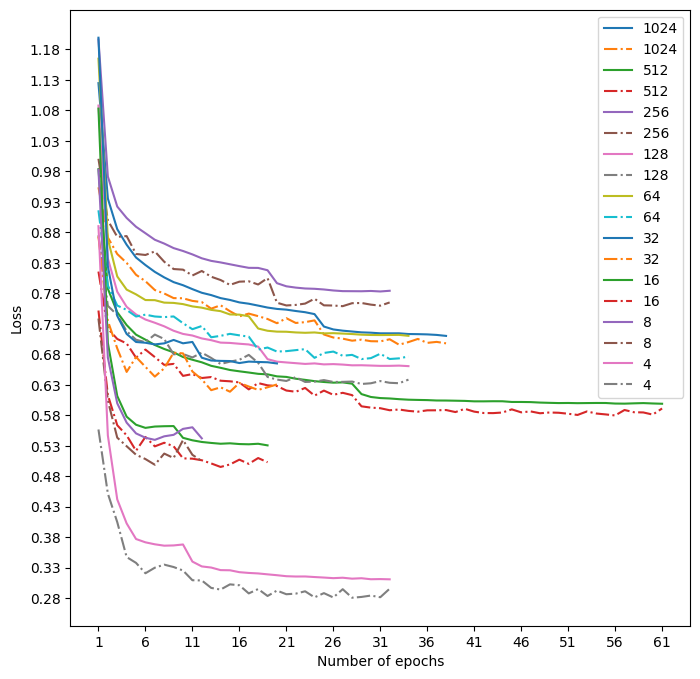
\includegraphics[width=300pt,height=300pt]{pictures/loss_dgcnn.png}
  \caption{Overview of the training and validation loss of the models trained with different values of dimension of the latent space representation when the number of nearest neighbors is fixed to 20. The y-axis represents the loss. The x-axis represents the number of epochs. The solid lines represent the mean training loss after each epoch. The dash dot line represents the mean validation loss after each epoch. The numbers in the legend represent the dimension of the latent space representations.}
  \label{fig:loss_dgcnn}
\end{figure} 

The model requires a training time of 70 hours for 19 epochs until convergence. The performance of the model is quite comparable to the model with dimension 64. Further reducing the dimension of the latent space representations degrades the performance of the models even more. Fig. \ref{fig:loss_dgcnn} gives an overview of all the models trained with \ac{DGCNN} as the backbone of the model for different sizes of the latent space representation. It can be observed that the validation loss is least when the model has dimensionality 4. But looking into the performance of the model while clustering the dataset, it can be seen that the performance is significantly worse. This could be a result of overfitting of the model. In the absence of enough dimensions of the latent space representations, the model is not properly calibrated. It learns the noise in the training dataset which makes it more confident in the predictions in the validation set which reduces the loss. But these "confident" predictions are actually incorrect predictions. Thus, there is a significant decrease in performance while clustering the dataset. Tab. \ref{tab:dgcnn_4} records the performance of the model when the dimensionality of the latent space representations is set to 4. 

\subsubsection{Evaluation of the effect of increasing datapoints} 
It is important to check that the results obtained on a small subset of the entire dataset can be relied upon for deriving conclusions on the entire dataset. Tab. \ref{tab:dgcnn_512} on Pg. 75 already shows the results of the model for 1000 datapoints.
\begin{table}[H]
  \setlength\extrarowheight{10pt}
  \caption{Results of the ConClu approach with \ac{DGCNN} backbone on 2000 datapoints when the dimension of the latent space representation is 512.}
  \centering
  \begin{tabular}{|p{30pt}|p{50pt}|p{60pt}|p{50pt}|p{50pt}|p{50pt}|p{40pt}|}
    \toprule
    \ac{t-SNE} dim	& \ac{t-SNE} time & Clustering Algorithm & No. of Clusters & Clustering Time (seconds) & \ac{DBCV} score & \ac{DBCV} Time (seconds)\\
    \midrule
    \multirow{4}{30pt}{2}	& 7.034	& \ac{HDBSCAN}	& 591	& 0.225	& 0.182	& 3.596.855 \\ \cline{2-7} 
    & 6.511	& k-medoids	& 175	& 0.213	& -0.202	& 409.159 \\ \cline{2-7} 
    & 6.730	& Spectral	& 175	& 26.729	& -0.129	& 410.735 \\ \cline{2-7}
    & 6.666	& Agglomerative	& 175	& 0.102	& -0.17	& 399.792 \\ 
    \bottomrule
  \end{tabular}
  \label{tab:dgcnn_2000}
\end{table}

Tab. \ref{tab:dgcnn_2000} records the performance of the model when the number of datapoints are increased to 2000. It can be seen that the time for dimensionality reduction with \ac{t-SNE} increases linearly on increasing the number of datapoints. But as mentioned earlier, the time for calculating the \ac{DBCV} score increases exponentially and not linearly. Similar to the observations with the PointNet autoencoder as backbone, the performance increases for the \ac{HDBSCAN} algorithm but not quite for the rest of the algorithms. This is because of the fact that more datapoints invariably mean more dense clusters when the number of clusters remain constant. Also, the \ac{DBCV} score  being a density based clustering validation index shows a better score for density based clustering algorithms. 

\begin{table}[H]
  \setlength\extrarowheight{10pt}
  \caption{Results of the ConClu approach on 2000 datapoints for multi-level \ac{HDBSCAN} clustering algorithm when the dimension of the latent space representation is 512. }
  \centering
  \begin{tabular}{|l|l|l|l|l|l|}
    \toprule
    Level & Algorithm	& No. of Clusters	& No. of Outliers	& DBCV score	& \ac{DBCV} time (seconds)	\\  
    \midrule
    Level 1 & \ac{HDBSCAN} & 591	& 193	& 0.129	& 327.926 \\ \cline{1-6}
    Level 2 & \ac{HDBSCAN} & 223	& 73	& -0.054	& 604.703
    \\ 
    \bottomrule
  \end{tabular}
  \label{tab:dgcnn_2000_levels}
\end{table} 

\begin{table}[H]
  \setlength\extrarowheight{10pt}
  \caption{Results of the ConClu approach with \ac{DGCNN} backbone on 5000 datapoints when the dimension of the latent space representation is 512. }
  \centering
  \begin{tabular}{|p{30pt}|p{50pt}|p{60pt}|p{50pt}|p{50pt}|p{40pt}|p{50pt}|}
    \toprule
    \ac{t-SNE} dim	& \ac{t-SNE} time & Clustering Algorithm & No. of Clusters & Clustering Time (seconds) & \ac{DBCV} score & \ac{DBCV} Time (seconds)\\
    \midrule
    \multirow{4}{30pt}{2}	& 17.516	& \ac{HDBSCAN}	& 1.486	& 0.647	& 0.185	& 120280.203 \\ \cline{2-7} 
    & 18.025	& k-medoids	& 175	& 0.550	& -0.409	& 2.696.609 \\ \cline{2-7} 
    & 6.730	& Spectral	& 175	& 26.729	& -0.129	& 410.735 \\ \cline{2-7}
    & 6.666	& Agglomerative	& 175	& 0.102	& -0.17	& 399.792 \\ 
    \bottomrule
  \end{tabular}
  \label{tab:dgcnn_5000}
\end{table}

\begin{table}[H]
  \setlength\extrarowheight{10pt}
  \caption{Results of the ConClu approach on 5000 datapoints for multi-level \ac{HDBSCAN} clustering algorithm when the dimension of the latent space representation is 512. }
  \centering
  \begin{tabular}{|l|l|l|l|l|l|}
    \toprule
    Level & Algorithm	& No. of Clusters	& No. of Outliers	& DBCV score	& \ac{DBCV} Time (seconds)	\\  
    \midrule
    Level 1 & \ac{HDBSCAN} & 1486	& 510	& 0.185	& 120280.203 \\ \cline{1-6}
    Level 2 & \ac{HDBSCAN} & 609	& 176	& -0.026	& 20.460.755 \\ \cline{1-6}
    Level 3 & \ac{HDBSCAN} & 265	& 106	& -0.205	& 4595.876 \\
    \bottomrule
  \end{tabular}
  \label{tab:dgcnn_5000_levels}
\end{table} 

Tab. \ref{tab:dgcnn_2000_levels} shows the performance of multi-level \ac{HDBSCAN} algorithm on this model. Tab. \ref{tab:dgcnn_5000} records the performance of the model when the number of datapoints are further increased to 5000. Tab. \ref{tab:dgcnn_5000_levels} shows the performance of multi-level \ac{HDBSCAN} algorithm on this model. As the number of datapoints increase, the number of iterations of the multi-level \ac{HDBSCAN} algorithm requires to reach a total number of clusters less than or equal to 175 also increases. Hence, it requires 3 levels for 5000 objects. It is to be noted that the performance of the multi-level \ac{HDBSCAN} algorithm improves with increase in the number of datapoints. 

\subsection{Comparison Between the PointNet Autoencoder Backbone and the Dynamic Graph Convolutional Neural Network backbone}

As observed earlier, the training time for the model with \ac{DGCNN} as the backbone is quite higher as compared to the models with PointNet autoencoder as backbone. And even with higher training time, the performance of the models are significantly worse. Amongst the models with \ac{DGCNN} as the backbone, the one with dimensionality 512 has the best results. But it requires a training time of 231 hours (i.e. almost 10 days) as compared to the model with PointNet autoencoder as backbone which requires 28 hours. Thus, fine-tuning the model for the rest of the hyperparameters with the \ac{DGCNN} backbone when the dimensionality is 512 is infeasible within the duration of this thesis as is possible for the model with PointNet autoencoder backbone, the results of which are recorded in Ch. \ref{sec:conclu_with_pointnet}. An overview of the training of the two models with different backbone but same dimensionality of the latent space representations is shown in Fig. \ref{fig:loss_camparison}. It can be observed that the ultimate validation loss for both the models are extremely comparable where the model with PointNet autoencoder backbone converges faster than the one with \ac{DGCNN} backbone. Thus, it seemed to be a rather practical choice to fine-tune the former model for the ultimate goal of this thesis. 

\begin{figure}[H]
  \centering
  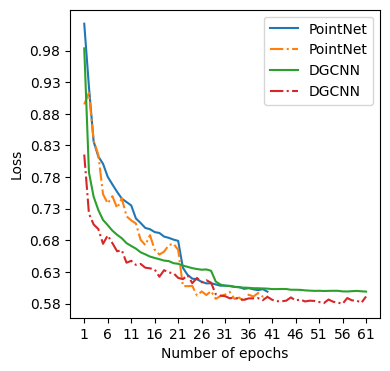
\includegraphics[width=300pt,height=300pt]{pictures/loss_comparison.png}
  \caption{Overview of the training and validation loss of the models trained with different backbones - PointNet autoencoder and \ac{DGCNN} when the dimension of the latent space representation is set to 512. The y-axis represents the loss. The x-axis represents the number of epochs. The solid lines represent the mean training loss after each epoch. The dash dot line represents the mean validation loss after each epoch. The legend represent the backbone of the model. }
  \label{fig:loss_camparison}
\end{figure}

\subsubsection*{Calculating the Similarity of the Test Dataset with the Representative Objects}

Once the representative objects are obtained, it is necessary to compare how similar they are compared to the objects in the test dataset. Hausdorff distance is commonly used to calculate the similarity between two point clouds.

\begin{table}[H]
  \setlength\extrarowheight{10pt}
  \caption{Similarity metric for the ConClu approach with PointNet Autoencoder backbone.}
  \centering
  \begin{tabular}{|p{50pt}|p{50pt}|p{50pt}|p{60pt}|p{50pt}|}
    \toprule
    Dataset Size(Whole)	& No. of  representative objects	& Dataset Size(Test)	& Clustering Algorithm	& Average Hausdorff Distance\\
    \midrule
    949647	& 94	& 49981	& multi-level \ac{HDBSCAN} &  0.170 \\ \cline{1-5} 
    949647	& 175	& 49981	& k-medoids	& 0.134 \\ \cline{1-5}
    949647	& 175	& 49981	& Spectral	&	0.155  \\ \cline{1-5}
    949647	& 175	& 49981	& Agglomerative	& 0.138 \\   
    \bottomrule
  \end{tabular}
  \label{tab:pointnet_sim}
\end{table}

 Table- \ref{tab:pointnet_sim} shows the similarity metric of the ConClu approach with the PointNet Autoencoder as backbone. It can be seen that the k-medoids has the minimum Hausdorff distance which is quite comparable to agglomerative clustering followed by spectral clustering and eventually multi-level \ac{HDBSCAN} algorithm. This can be due to the fact that the traditional spectral clustering algorithm and agglomerative clustering doesn't give medoids of the cluster but cluster centres. But to ensure that the cluster centres are actual members of the dataset, Hausdorff distance is used to calculate the medoid of the clusters from the respective cluster members.  Because of this usage of Hausdorff distance in calculating the medoid, it is possible that when Hausdorff distance is used to calculate the ultimate similarity of the test dataset and the representative members, it slightly favoured the clustering algorithm which already used it for calculating the cluster medoid. Also to make it consistent with spectral clustering and agglomerative clustering, Hausdorff distance is also used as the pairwise distance metric during the k-medoids. Overall, it is to be noted further that even if the average distance for multi-level \ac{HDBSCAN} is a little more  than the rest of the algorithm, the variation isn't quite drastic. Tab. \ref{tab:dgcnn_sim} shows the similarity metric of the ConClu approach with the \ac{DGCNN} as backbone. It is observed that the results for both the backbones are very similar. Hence, it is not conclusive enough to use just this similarity metric to choose a suitable network for the purpose. 

\begin{table}[H]
  \setlength\extrarowheight{10pt}
  \caption{Similarity metric for the ConClu approach with \ac{DGCNN} backbone.}
  \centering
  \begin{tabular}{|p{50pt}|p{50pt}|p{50pt}|p{60pt}|p{40pt}|}
    \toprule
    Dataset Size(Whole)	& No. of  representative objects	& Dataset Size(Test)	& Clustering Algo	& Average Hausdorff Distance\\
    \midrule
    949647	& 94	& 49981	& multi-level \ac{HDBSCAN} &  0.170 \\ \cline{1-5} 
    949647	& 175	& 49981	& k-medoids	& 0.133 \\ \cline{1-5}
    949647	& 175	& 49981	& Spectral	&	0.152  \\ \cline{1-5}
    949647	& 175	& 49981	& Agglomerative	& 0.137 \\   
    \bottomrule
  \end{tabular}
  \label{tab:dgcnn_sim}
\end{table}

\subsection{Results}

Observing the results of the experimentations it is evident that the \ac{HDBSCAN} algorithm has significantly better performance as compared to any other clustering algorithm. But it had a major drawback of not having any control on the ultimate number of clusters obtained in the end. To circumnavigate this issue, the idea of multi-level \ac{HDBSCAN} is proposed. This naturally degrades the \ac{DBCV} score to some extent because the least-dense region within a cluster is no longer more dense as compared to the region in-between clusters but it has 2 important benefits. It had a control on the ultimate number of representative objects of the dataset which is very crucial in the present use-case. Also often times, it is observed that even though the result of this algorithm is not up to the mark as of \ac{HDBSCAN} algorithm, it is still better or at  least comparable to the next best algorithm, i.e. the spectral clustering algorithm. Furthermore, another significant benefit of multi-level \ac{HDBSCAN} algorithm as compared to spectral clustering is that the latter takes significantly higher time to cluster such a large dataset as compared to the former. Even in evaluations recorded in Ch. \ref{sec:experiments} it can be seen that the time taken by the spectral clustering algorithm is quite high as compared to any other algorithm. The multi-level \ac{HDBSCAN} algorithm takes 0.8 seconds to cluster 1000 datapoints, whereas spectral clustering takes 7.2 seconds for the same task. This phenomenon is even intensified when the number of samples increase from 1000 datapoints to 1 million datapoints. Spectral clustering takes roughly 20 days to form 175 clusters from the entire dataset, whereas the multi-level \ac{HDBSCAN} takes as less as 3 hours. This is because spectral clustering has a time complexity of $O(N^3)$ for a dataset with $N$ objects. Also, it is observed that the multi-level \ac{HDBSCAN} algorithm had better performance in most cases as compared to spectral clustering. Thus, it is inefficient to use such large clustering time for worse performance. The ultimate goal of this thesis is to identify "good" source data that represents the variance of the entire dataset.

\begin{figure}[t]
  \centering
  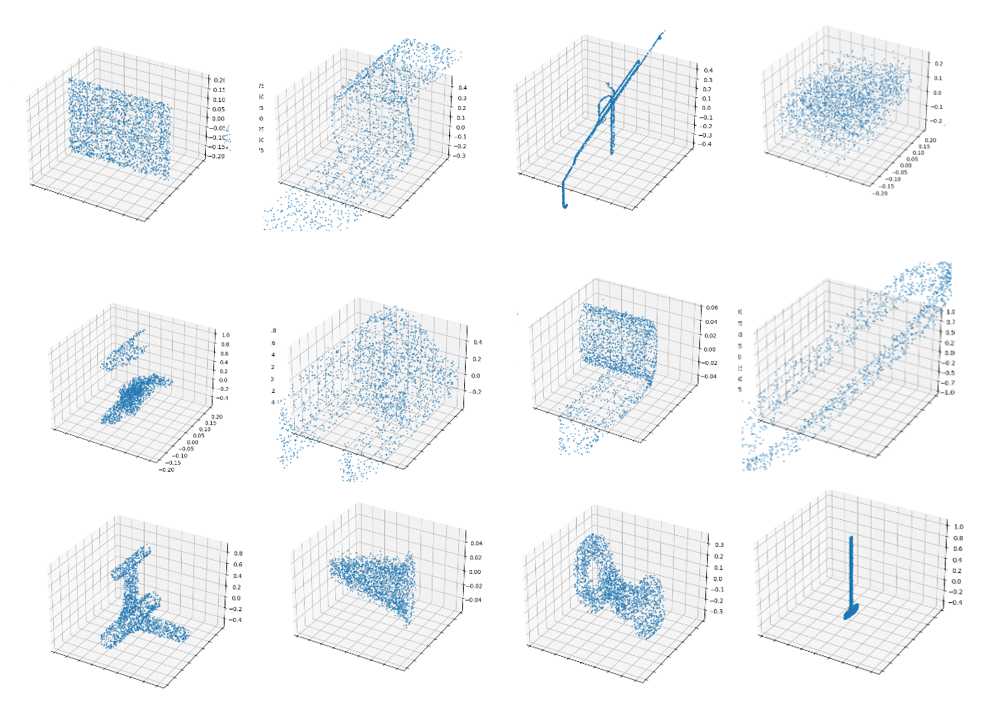
\includegraphics[width=400pt,height=300pt]{pictures/all_objs.PNG}
  \caption{Some of the representative members of the ABC dataset\cite{Koch_2019_CVPR} obtained on applying multi-level \ac{HDBSCAN} algorithm on the feature representations obtained from the ConClu approach with PointNet Autoencoder backbone.}
  \label{fig:all_hdbscan_objs}
\end{figure}

It is observed that the objects obtained after the applying the clustering algorithms are quite diverse in nature. Although there is no known objective way to determine what qualifies as a "good" source object in case of unsupervised learning, the diversity in the objects obtained in the end quite ensures the fulfillment of the task in hand. Fig. \ref{fig:all_hdbscan_objs} shows some of the cluster representatives obtained after applying the multi-level \ac{HDBSCAN} algorithm. Only some objects were chosen from the entire set of representative objects for the sake of visualization. It can be seen that the representative objects of the dataset are quite diverse in nature. Ranging from an ellipse shaped ring, an aircraft to a dumbbell, the objects are quite different from one another. Thus, weighing the pros and cons of the two different backbones and the 5 different clustering algorithm, it can be concluded that the ConClu approach with the PointNet Autoencoder gives the best model for the generation of the latent space representations of te objects in the dataset. Furthermore, weighing the performance of the clustering algorithm under different setup and the overall time required by the clustering algorithms, the multi-level \ac{HDBSCAN} algorithm seems to be a practical choice for this scenario. The \ac{HDBSCAN} algorithm has better performance compared to the multi-level \ac{HDBSCAN} algorithm because more number of clusters would naturally mean more smaller but denser clusters. But since it has no control on the number of clusters it returns and mostly returns a large number of clusters in the presence of a large dataset. Having such a high number of cluster representatives isn't feasible for further tasks in the current setup at \ac{IPA}. This is why the maximum number of cluster representatives is set to 175. Under this particular constraint, the multi-level \ac{HDBSCAN} algorithm is the best choice for clustering algorithm in this use-case. 
\cleardoublepage